\documentclass[letterpaper]{article}
\usepackage{natbib,alifeconf}
\usepackage[breaklinks=true]{hyperref}
\usepackage{url}

\graphicspath{{../img/}}
\DeclareGraphicsExtensions{.pdf}

\title{The human in the loop: volunteer computing as a socio-technical
system}
\author{Juan-J.~Merelo*$^1$, Paloma de las Cuevas $^1$, Pablo
  Garc\'ia-S\'anchez $^1$, Mario Garc\'ia-Valdez$^2$\\
\mbox{}\\
$^1$Dept. of Computer Architecture and Technology and CITIC University of Granada \\
$^2$Dept. of Graduate Studies at Instituto Tecnol\'ogico de Tijuana \\
{\tt jmerelo@ugr.es}, {\tt mario@tectijuana.edu.mx}}

\begin{document}
\maketitle

\begin{abstract}
Volunteer computing is a form of distributed computing where users
decide on their participation and the amount of time and other resources they will
``lend''. This makes them an essential part of the algorithm and of
the performance of the whole system. As a sociotechnical system, this
participation follows some patterns and in this paper we examine the
result of several volunteer distributed evolutionary computation
experiments and try to find out which are those patterns and what
makes an experiment successful or not, including the feedback loop
that is created between the users and the algorithm itself. In this
paper we will examine what kind of patterns we can expect and what
influence those patterns have on the implementation of the
evolutionary algorithm. 
%Pablo: The patterns we are looking for are... 
\end{abstract}

\section{Introduction}
\label{introduction}

Some time ago, our group faced the problem of diminishing funds for
buying new hardware. This was aggravated by the increasing maintenance
costs and extended downtime resulting from the continuous failures of
existing clusters.  Considering this, we leveraged our experience in
the design of web applications with JavaScript and other volunteer and
unconventional distributed evolutionary computing systems to design
and release a new free framework that would allow anyone to create a
volunteer distributed evolutionary computation (EC) experiment using
cloud resources as servers and browsers as clients. This framework was
called NodIO \citep{2016arXiv160101607M}. NodIO provides server
infrastructure for volunteer-based distributed evolutionary computing
experiments by providing a chromosome {\em pool}. This pool is used by
clients in browsers and any other using the application programming
interface (API) to put chromosomes and retrieve them, working then as
a loose, asynchronous and {\em ad hoc} connection among all clients
using it. 

This loose connection provides a low-overhead way to connect desktop
experiments with volunteer-based ones, with all of them contributing
to the pool, but every one of them working as separate island 
carrying out their own evolutionary algorithms. This is why NodIO is
proposed mainly as a {\em complement} to existing resources such as
desktop systems or laptops. As long as it provides a non-null
computational capability that can help existing resources find the
solution faster it will have found its purpose. The main use case is
someone setting up NodIO in the cloud, writing a fitness evaluation
function and running a client from his or her own computer, but
requesting help in social networks for additional resources. That is
why, in this system,  we have considered the whole {\em social} aspect
in the design, with issues related to security, trust and privacy
among others. The computing system becomes a {\em techno-social
%Pablo: In abstract is named 'sociotechnical'. Which one is the correct form for the rest of the paper?
  system} \citep{vespignani2009predicting}. In this paper, we are going
to focus on measuring the response of users to experiments, but at the
%Pablo: which metric are we going to measure this response?
same time we will also focus on the technical aspects of the server and how
those might change the behavior of users, improving the capability of % Mario: How these might change
the system.

Our research group is committed to open science, and we think this is
a very important part of the techno-social system. By being
transparent, incentives to cheat are reduced and, in fact, we have
detected no issue for the time being. Next we present the state of the art in web-based
volunteer-based systems along with attempts to predict and model its
behavior. 


%---------------------------------------------------------------
\section{State of the art}
\label{sec:soa}

Volunteer computing involves a user running a program voluntarily
and, as such, has been deployed in many different ways from the
beginning of the Internet, starting with the SETI@home framework for
processing extraterrestrial signals \citep{david-seti:home}. However
the dual introduction of JavaScript as a universal language for the
browser and the browser as an ubiquitous web and Internet client has
made this combination the most popular for volunteer computing
frameworks such as the one we are using here, and whose first version
was described in \citep{DBLP:conf/gecco/GuervosG15}.

JavaScript can be used for either unwitting
\citep{unwitting-ec,boldrin2007distributed} or volunteer 
\citep{langdon:2005:metas,gecco07:workshop:dcor} distributed
evolutionary computation and it has been used ever since by several
authors, including more recent efforts
\citep{Desell:2008:AHG:1389095.1389273,duda2013distributed,DBLP:journals/corr/abs-0801-1210}. Many other researchers have
%Pablo: Desell in 2008 is not so recent
used Java \citep{chong:1999:jDGPi} and others have gone away from the
server-based paradigm to embrace peer to peer systems
\citep{jin2006constructing,10.1109/ICICSE.2008.99,DBLP:conf/3pgcic/GuervosMFEL12}. These computing
platforms avoid single points of failure (the server) but, since they
need a certain amount of infrastructure installed to start, the
threshold to join them is much lower; this makes gathering new users
immediate and spontaneous, so that they can be used for short
algorithms on call.


On the other hand, we are also interested in measuring the performance
of volunteer computing systems, an area in which there have been
relatively few efforts.
There were some initial attempts to avoid the differences in performance
that could be obtained from volunteers  by making
the algorithm adaptive to the kind of resources allotted to it
\citep{milani2004online}, which is actually not such a big problem in
algorithms such as the EA that can be easily 
parallelized via population splitting or by farming out the evaluation to all
the nodes available. Lately, several approaches have focused on the
fault-tolerance of volunteer systems
\citep{gonzalez2010characterizing} which it can, of course, be studied in
the more general context of distributed computing 
\citep{nogueras2015studying} or including it in a more general study of the
performance of the EA itself
\citep{DBLP:journals/gpem/LaredoBGVAGF14}. This performance cannot be
measured without first understanding the dynamics of this kind of systems. Initial
work was done for peer to peer systems by Stutzbach et
al. \citep{stutzbach2006understanding} and extended to volunteer
computing by Laredo et al. \citep{churn08,laredo2008rcp}. A similar
study was performed by Martínez et al. on the Capataz system
\citep{martinez2015capataz}; however, in this case the number of
computers used was known in advance and the main focus was on
measuring the speed up and how job bundling helped to reduce overhead and
enhance performance. On the contrary, in this paper, we will use {\em
  actual} volunteers, anonymous persons that are requested to join an
experiment through social networks.

Some of the essential metrics in volunteer computing like the
number of users or the time spent by every one in the
computation in browser-based volunteer computing experiments, have
only been studied in a limited way in 
\citep{DBLP:journals/gpem/LaredoBGVAGF14} on the basis of a single
run. Studies using volunteer computing platforms such as SETI@home
\citep{javadi2009mining,agajaj} found out that the Weibull, log-normal and
Gamma distribution 
modeled quite well the availability of resources in several clusters
of that framework; the shape of those distributions is a skewed bell
with more resources in the {\em low} areas than in the high areas:
there are many users that give a small amount of cycles, while there
are just a few that give many cycles. 

As far as we know, this paper presents one of the few experiments
that measure the performance of a sociotechnical
metacomputer, that is, a spontaneously created parallel computer that
uses social networks for operations such as gathering new
users. Apol{\'o}nia et al. \citep{apolonia2012enhancing} used the 
Facebook protocol to distribute tasks among the {\em walls} of
friends, explicitly using the social network for computing. However,
it stopped short of relating performance to the macro measures of the
users' social networks. As in the previous example, a social network
was used to get new network nodes; in the previous case a web page was
used, while Facebook's wall was used here.
The algorithms used, as well as the methodology 
for gathering resources will be described next, 
together with the results obtained in this initial setup.


\section{Description of the framework}
\label{sec:description}

In general, a distributed volunteer-based evolutionary computation
system based on the browser is simply a client-server system
whose client is, or it can be, embedded in the browser via
JavaScript. Since JavaScript is  the only language that is present
across all browsers, the choice was quite clear. We should emphasize
that NodIO is more intended as an auxiliary computing engine, more
than the main one, so performance of JavaScript as a language is not
so important; even so, we have made a comparison between JavaScript and other languages
\citep{2015arXiv151101088M} that shows that performance of JavaScript
is comparable to other interpreted languages; compiled languages would
be faster, but, of course, it is impossible to gather volunteers
spontaneously and without any installation with them.

In this sense, in this paper we propose the {\sf NodIO} framework, a
cloud or bare metal based volunteer evolutionary computing system
derived from the {\sf NodEO} library, whose architecture has been
developed using JavaScript on the client as well as the server.
All parts of the framework are free and available with a free license
from \url{https://github.com/JJ/splash-volunteer}.

Thus, {\sf NodIO} architecture has two tiers:\begin{enumerate}
\item A REST server, that is, a server that includes several {\em
  routes} 
  that can be called for storing and retrieving information (the ''CRUD'' cycle:
  create, request, update, and delete) from the server. 
  A JSON data format is used for the communication between 
  clients and the server. There are two kinds of information:
  {\em problem} based, that is, related to the
  evolutionary algorithm such as {\tt PUT}ing a chromosome in or {\tt
  GET}ing a random chromosome from it, and {\em information} related
  to the performance and state of the experiments. It also performs logging
  duties, but they are basically a very lightweight and high performance
  data storage \citep{jj:idc:lowcost}.
  The server has the capability to
  run a single experiment, storing the chromosomes in a data structure
  that is reset when the solution is found. This data structure can
  hold every chromosome in a particular experiment, or have a finite
  size that erases the oldest chromosomes once it has filled to
  capacity. In this paper we will test both implementations.  
\item A client that includes the evolutionary algorithm as
  JavaScript code embedded in a web page that displays graphs, some
  additional links, and information on the experiment. This code runs
  an evolutionary algorithm {\em island} that starts with a random
  population, then after every 100 generations, it sends the best individual
  back to the server (via a {\tt PUT} request), and then requests a random
  individual back from the server (via a {\tt GET} request). We have
  kept the number of generations between migrations fixed since it is
  a way of finding out how many real work every client has done. 
\end{enumerate}

Figure \ref{fig:system} describes the general system architecture and
algorithm behavior. Different web technologies, such as JQuery or {\tt
  Chart.js} have
been used to build the user interface elements of the framework.


\begin{figure}[!t]
\centering
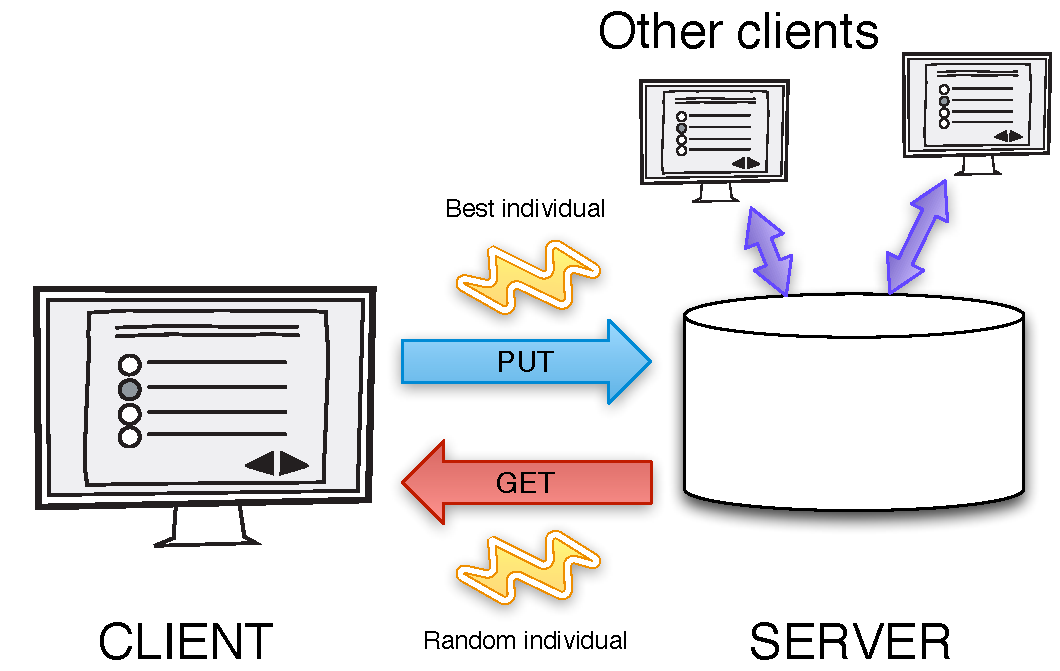
\includegraphics[width=3in]{system.pdf}
\caption{Description of the proposed system. Clients execute a JavaScript EA
  in the browser, which, every 100 generations, sends the best
  individual and receives a random one back from the server.}
\label{fig:system}
\end{figure}

In this case the classical Trap function \citep{Ackley1987} has been
used. JavaScript is a functional language and declaring a different 
function and handing at the creation of the algorithm object, called
{\tt Classic}, is the only change needed to work with a different
problem. The next Section will describe experiments performed to
establish baseline performance and gather initial performance
results. In the experiments performed last year we used the 40-trap
problem, while the current experiments changed to the more difficult 50-trap.

%---------------------------------------------------------------
\section{Modeling the performance of a volunteer-based distributed computer} 
\label{sec:experiments}

\begin{table}[htb]
\caption{Experiment table, with summary of results. \label{tab:runs}}
\begin{center}
\begin{tabular}{l|rrl}
\hline
Experiment & \#Runs & Different IPs & Traps \\
\hline
April 4th 4/4 & 57 & 191 & 40 \\
April 24th 4/24 &  231 & 559& 40  \\
July 31th 7/31 & 97 & 179 & 40 \\
\hline
February, cache=128 & 61 & 75 & 50  \\
February, cache=64 & 61 & 220 & 50  \\
February, cache=32 & 39 & 86 & 50  \\
% grep start ~/Code/splash-volunteer/data/2016/nodio-2016-2-28-cache=32.log
\hline
\end{tabular}
\end{center}
\end{table}
%
Initial experiments were set up using the OpenShift
PaaS, which provides a free tier, making the whole experiment cost
equal to 0. Experiments were
announced through a posts in Twitter and, the latest case, Telegram, and
results were published here \citep{DBLP:conf/gecco/GuervosG15}. For the
purpose of this paper, we repeated the announcement several times
through the month of April and then by the end of February. All
in all, we have the set of runs with the characteristics shown in
Table \ref{tab:runs}. In general, every experiment took several
days. No particular care was taken about the time of the announcement
or the particular wording. Every {\em experiment} consisted in running
until the solution of the 40-trap problem was found. When the correct
solution was sent to the server, the counter was updated and the pool
of solutions reset to the void set. There was no special intention to wait
until all clients had finished, thus it might happen that, in fact,
the islands running in the browser {\em spill} from one experiment to
the next. However, previous experiments have proven that the influence
of these islands in the next experiment is indeed negligible.


The table shows that every run included more than 30 experiments. The
number of different IPs intervening in them varied from more than one
hundred to more than five hundred in the second experiment, with a
number around 50 in the second, and most recent, batch of experiments. 
%
\begin{table}[htb]
\caption{Summary of time per run, number of IPs and number of {\tt
    PUT}s per IP in the initial runs. \label{tab:summary:os}}
\begin{center}
\begin{tabular}{l|cccc}
\hline
     & \multicolumn{2}{c}{IPs} & \multicolumn{2}{c}{Median} \\
Experiment & Median & Max & time (s) &  \#{\tt  PUT}s \\
\hline
4/4 & 5 & 16 & 2040 & 18   \\
4/24 &  5 & 29 & 732 & 11  \\
7/31 & 5 & 14 & 260 & 23   \\
\hline
Cache=128 & 5 & 17 & 222.2 & 124 \\ 
Cache=64 & 8 & 38 & 51.3 & 100 \\
Cache=32 & 6 & 19 & 58.9 & 45 \\
\hline
% Data in .RData file in Splash-volunteer
\end{tabular}
\end{center}
\end{table}
%

A summary of the results of each run is also shown in Table
\ref{tab:summary:os}, which shows the median number of IPs
intervening in each experiment,  median time needed
to finish the experiment, median number of HTTP {\tt PUT}s per IP. The
first striking result is that in all cases, 50\% of the 
experiments involved 5 or less IPs. This is consistent with previous results
\citep{DBLP:conf/gecco/GuervosG15} which found 6 to be
the expected number of volunteer IPs. The
maximum number of different IPs for each experiment is also in the
same range and of the order of 10, which is also consistent with
prior work and does not vary across the two different batches. 

We will have to analyze differently the median time, since the two
batches are solving different problems. In both cases it possesses a
big range of variation, but 50\% of 
the time takes less than several minutes, from around 4 minutes in the
best case to roughly 2/3 of an hour in the worst case. Remarkably
enough, the time is more consistent in the second batch and always
around one minute, in two cases even less, and that happens when the
median number of IPs is higher. It should be noted that while the
first batch of experiments took several days in each case, the second
only lasted for a few hours, with a more continued effort of
publicizing it in social networks; this is specially true in the
case of cache equal to 64, which is noticed by the high number of
volunteers participating in the experiment. The conclusion is that,
in general, the key factor in the time needed to find the solution
is, as expected, the number of volunteers it is able to gather on a
short notice. 

The number of {\tt PUTs}, every one corresponding to 100 generations,
is the algorithmic result. It is relatively unchanged for the first
batch and around 20, that is, 2000 generations or 2000*128 = 256000
evaluations. In this case, an ``unlimited'' cache was used, with all
individuals sent from clients stored until the end of the
experiment. However, we were interested in measuring also the
performance of the algorithm itself by changing the cache size, after
making it limited. As it can be seen in the table, there is a clear
change in the number of evaluations needed, with smaller cache sizes
producing solutions in less evaluations, until it is for the cache
size = 32 roughly twice as much as with the previous problem, with 40
traps. This is a good result and is also algorithmically consistent
with other results obtained using the same type of problems. Since in
this paper we were interested in leveraging the user's CPU cycles by
improving the algorithm, a good conclusion of this paper is that
having a small pool size helps clients to obtain ``good'' individuals
from the pool, as opposed to any individual that could be obtained
before. Besides, cache policy deletes the oldest individuals, which
makes those in the pool be {\em current}, helping then newcomers and
any participant obtain the best individuals found in the last part of
the experiment. Besides, a limited cache helps also in cases with a
bigger search space or longer running times when the server simply
crashed due to lack of RAM. 

\begin{figure}[!htb]
\centering
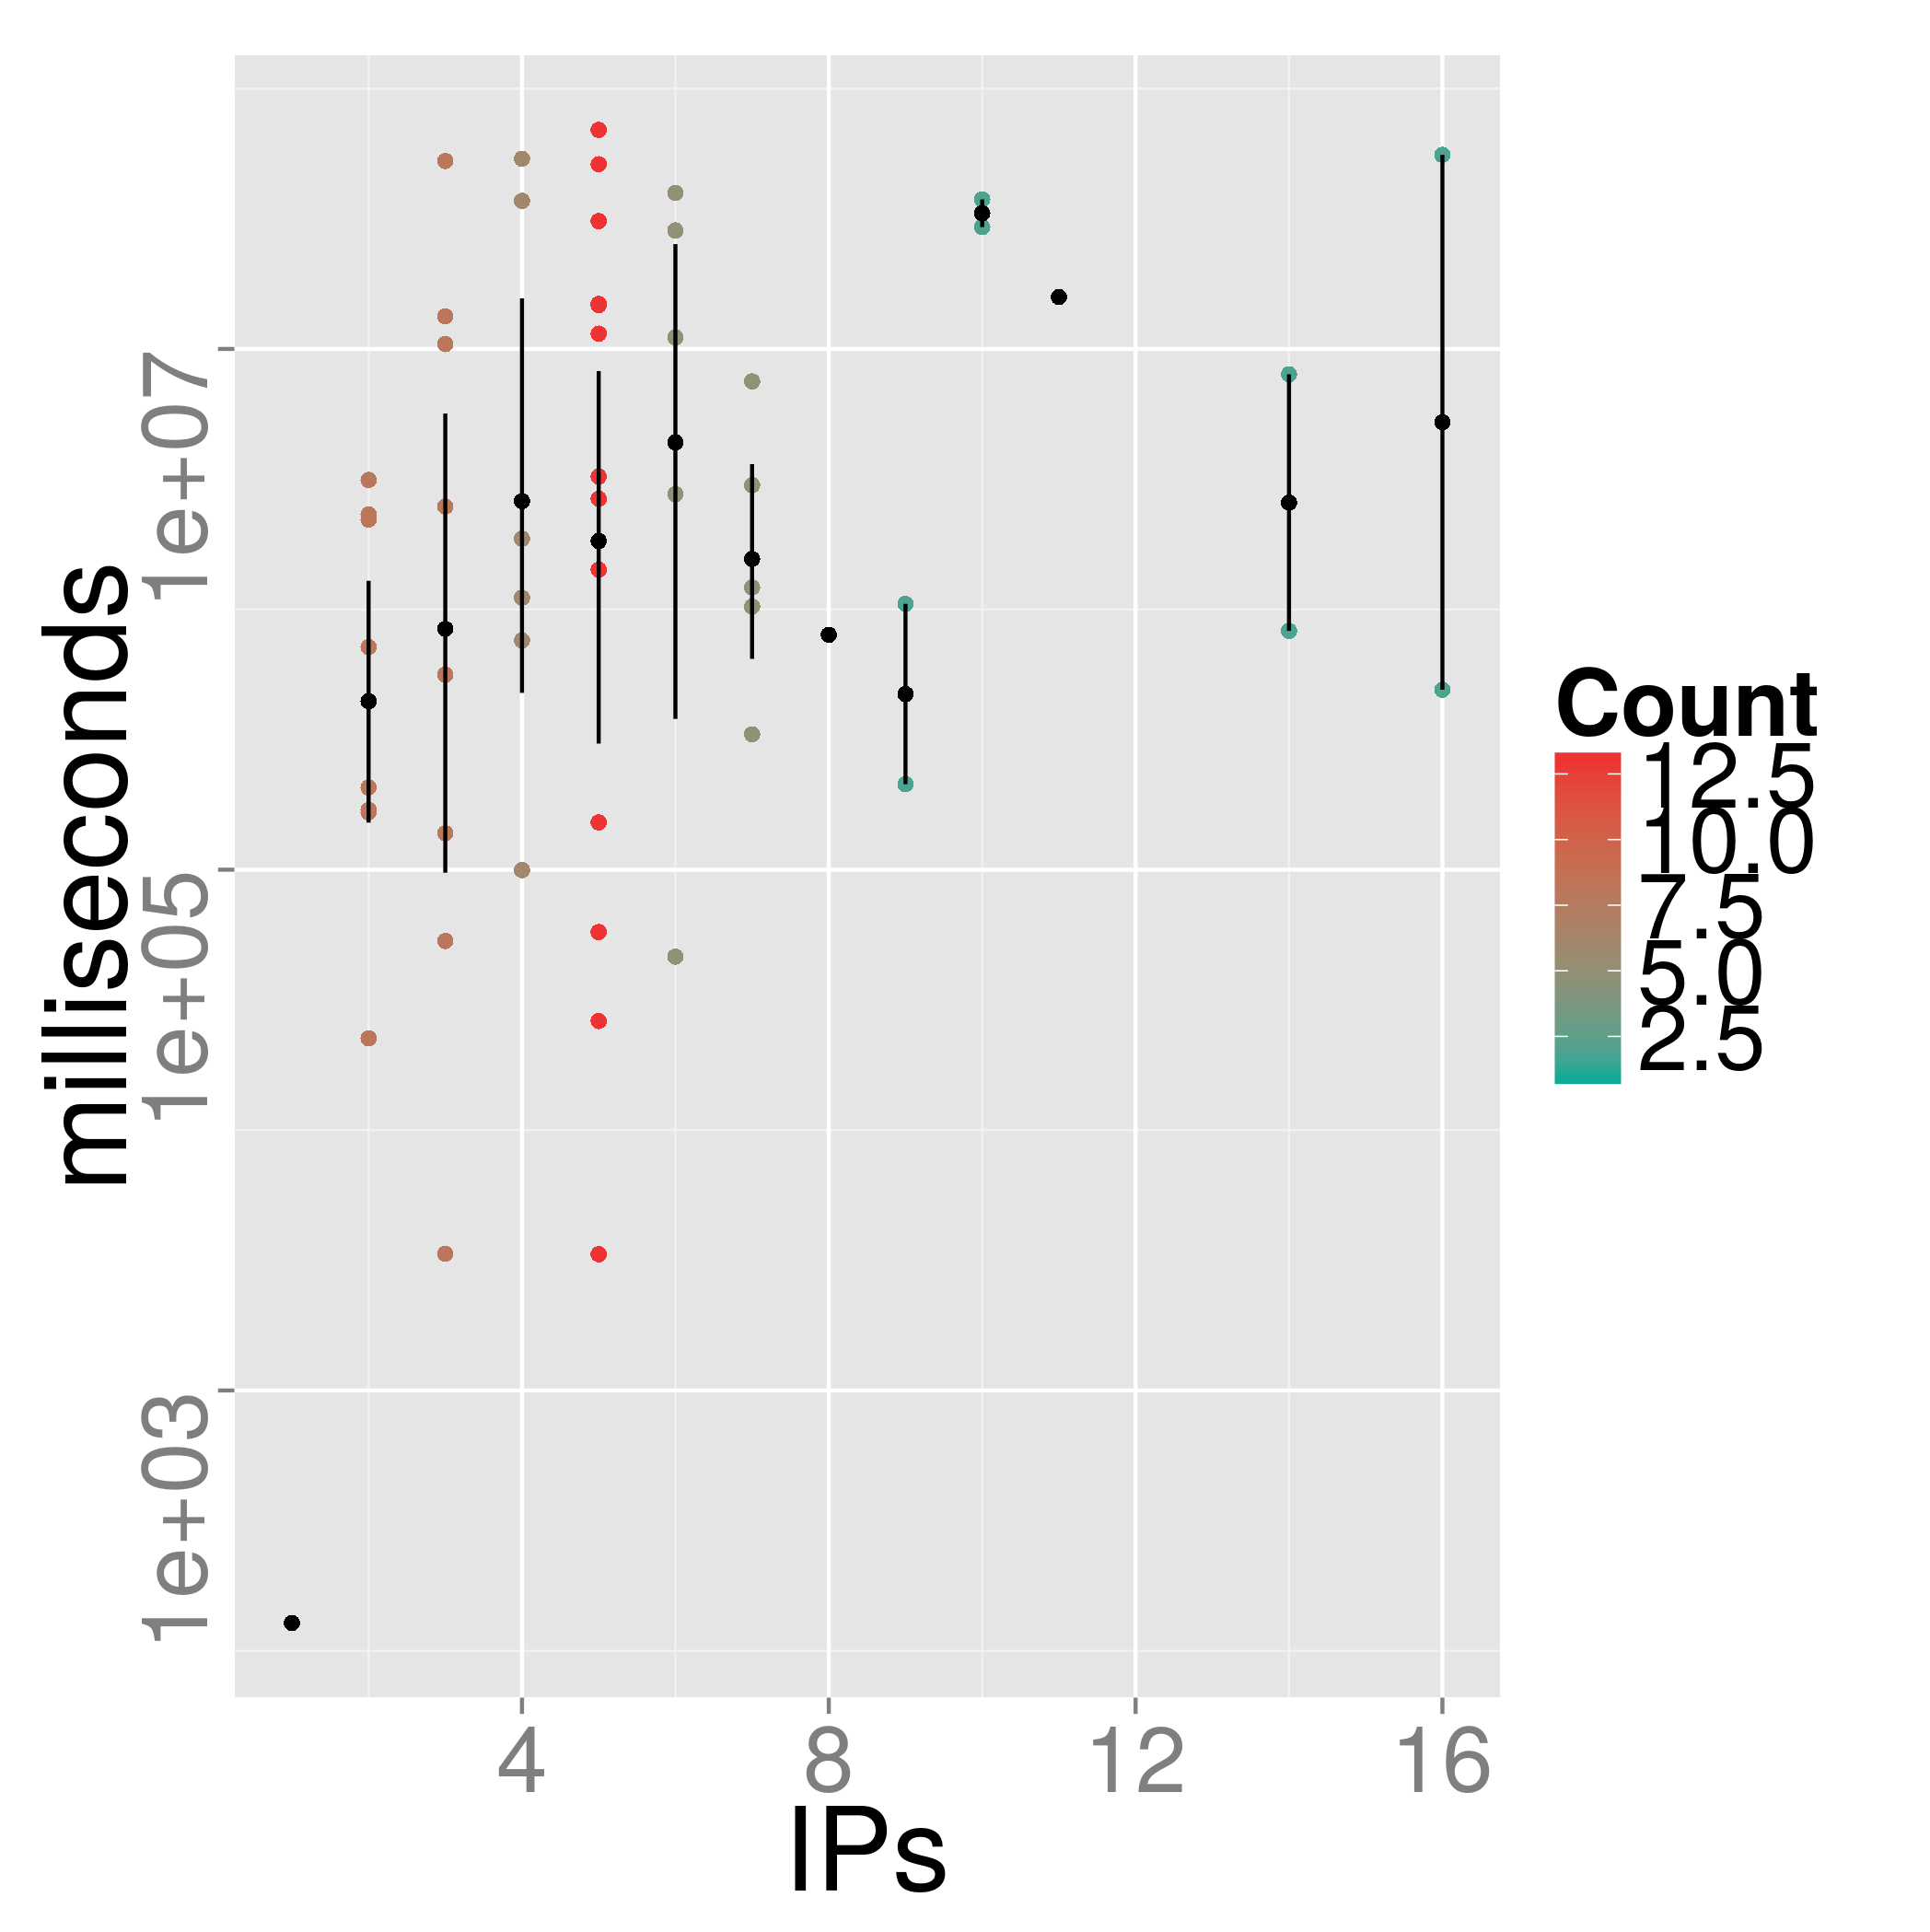
\includegraphics[width=0.32\linewidth]{time-vs-ips-OS-4-4.png}
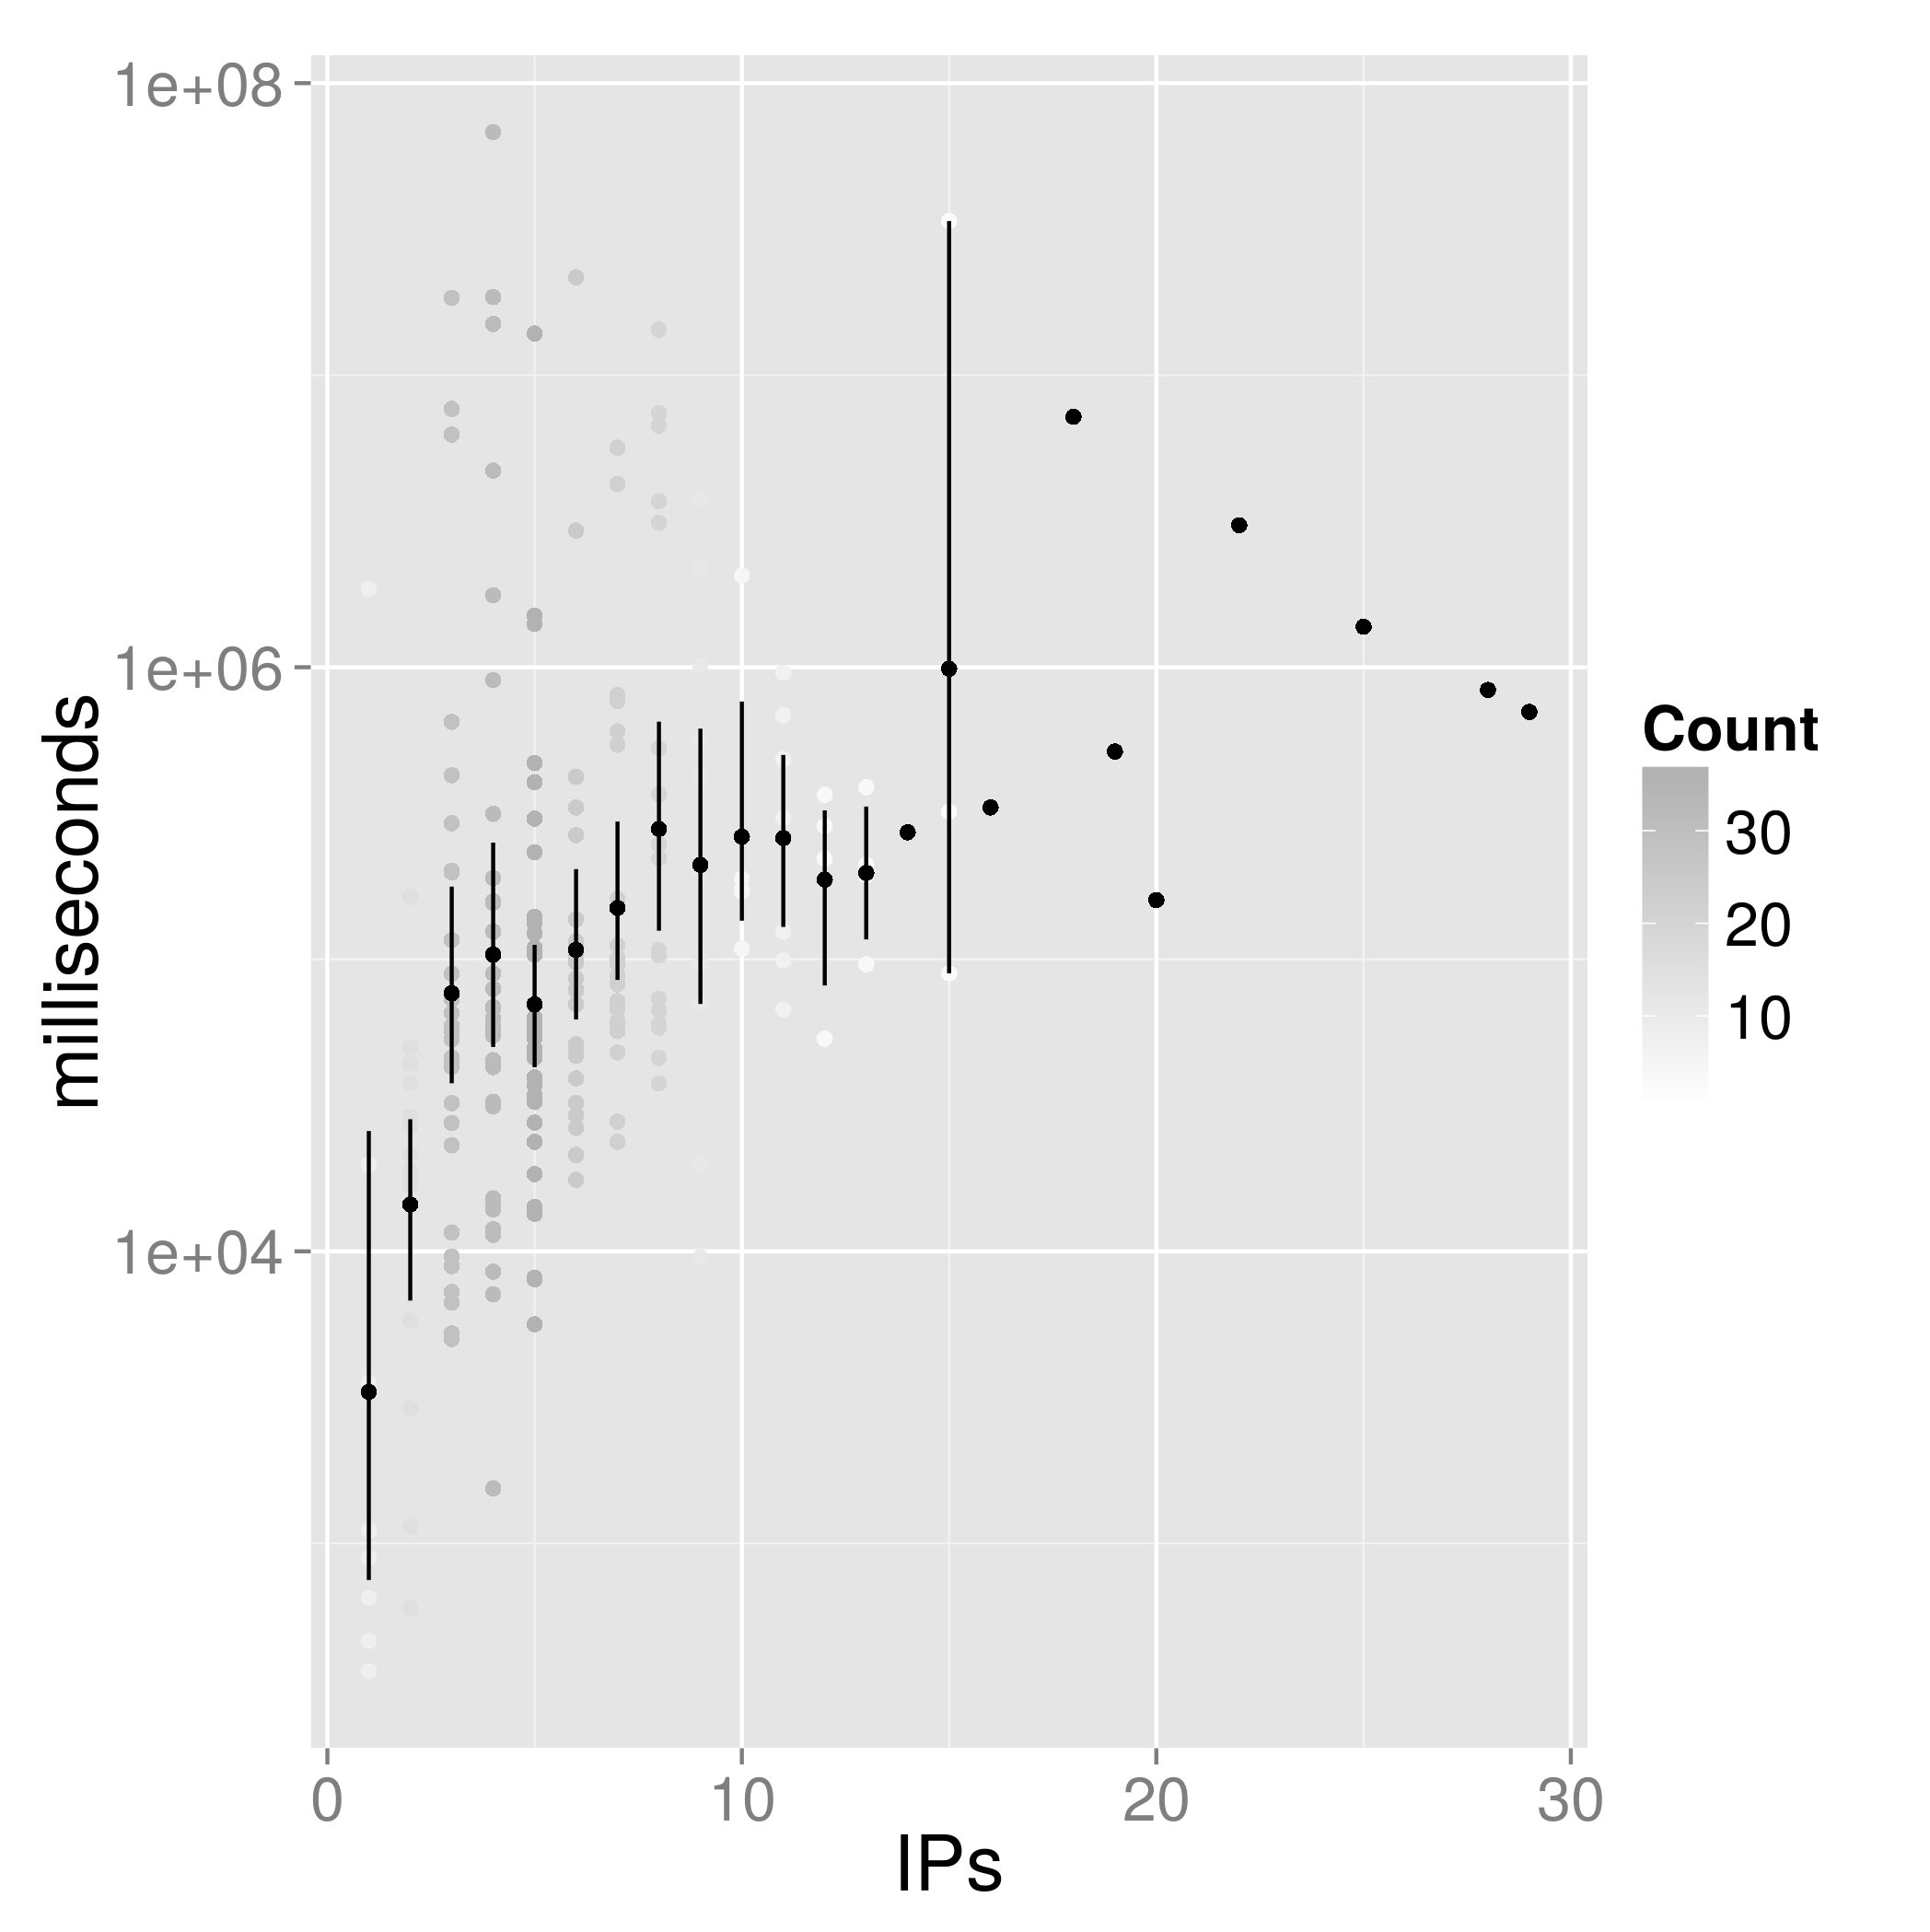
\includegraphics[width=0.32\linewidth]{time-vs-ips-OS-4-24.png}
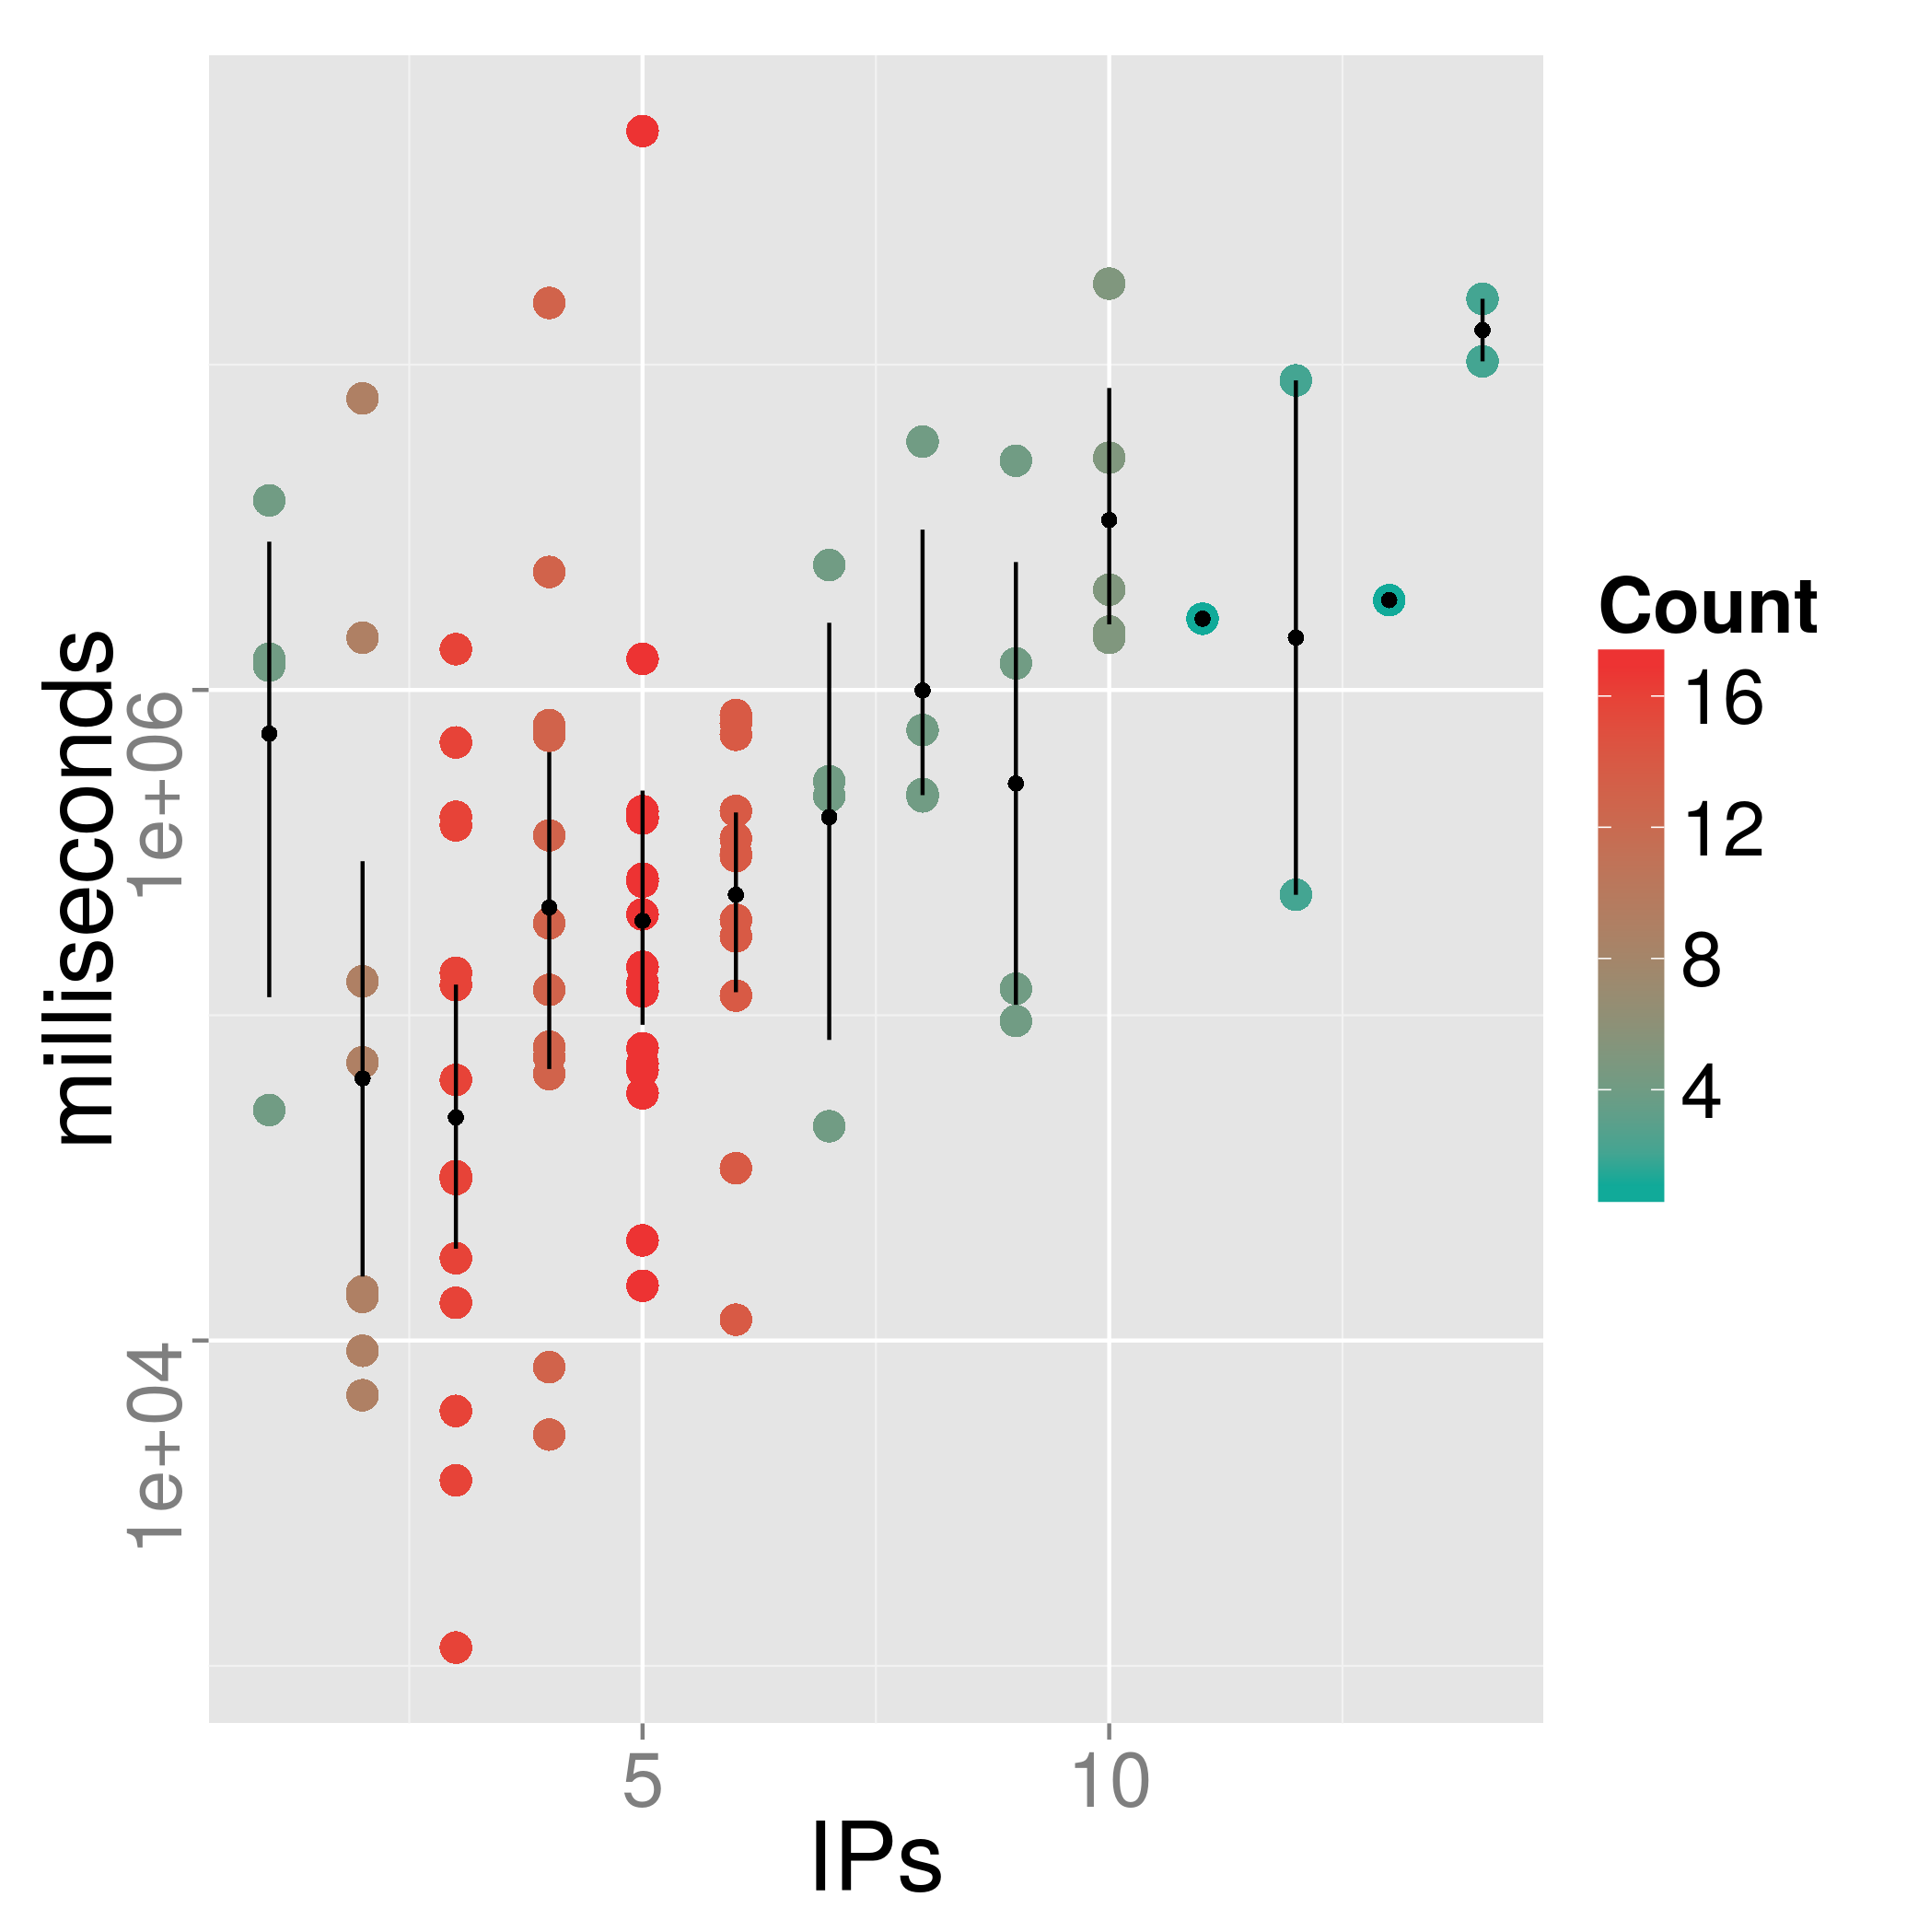
\includegraphics[width=0.32\linewidth]{time-vs-ips-OS-7-31.png}
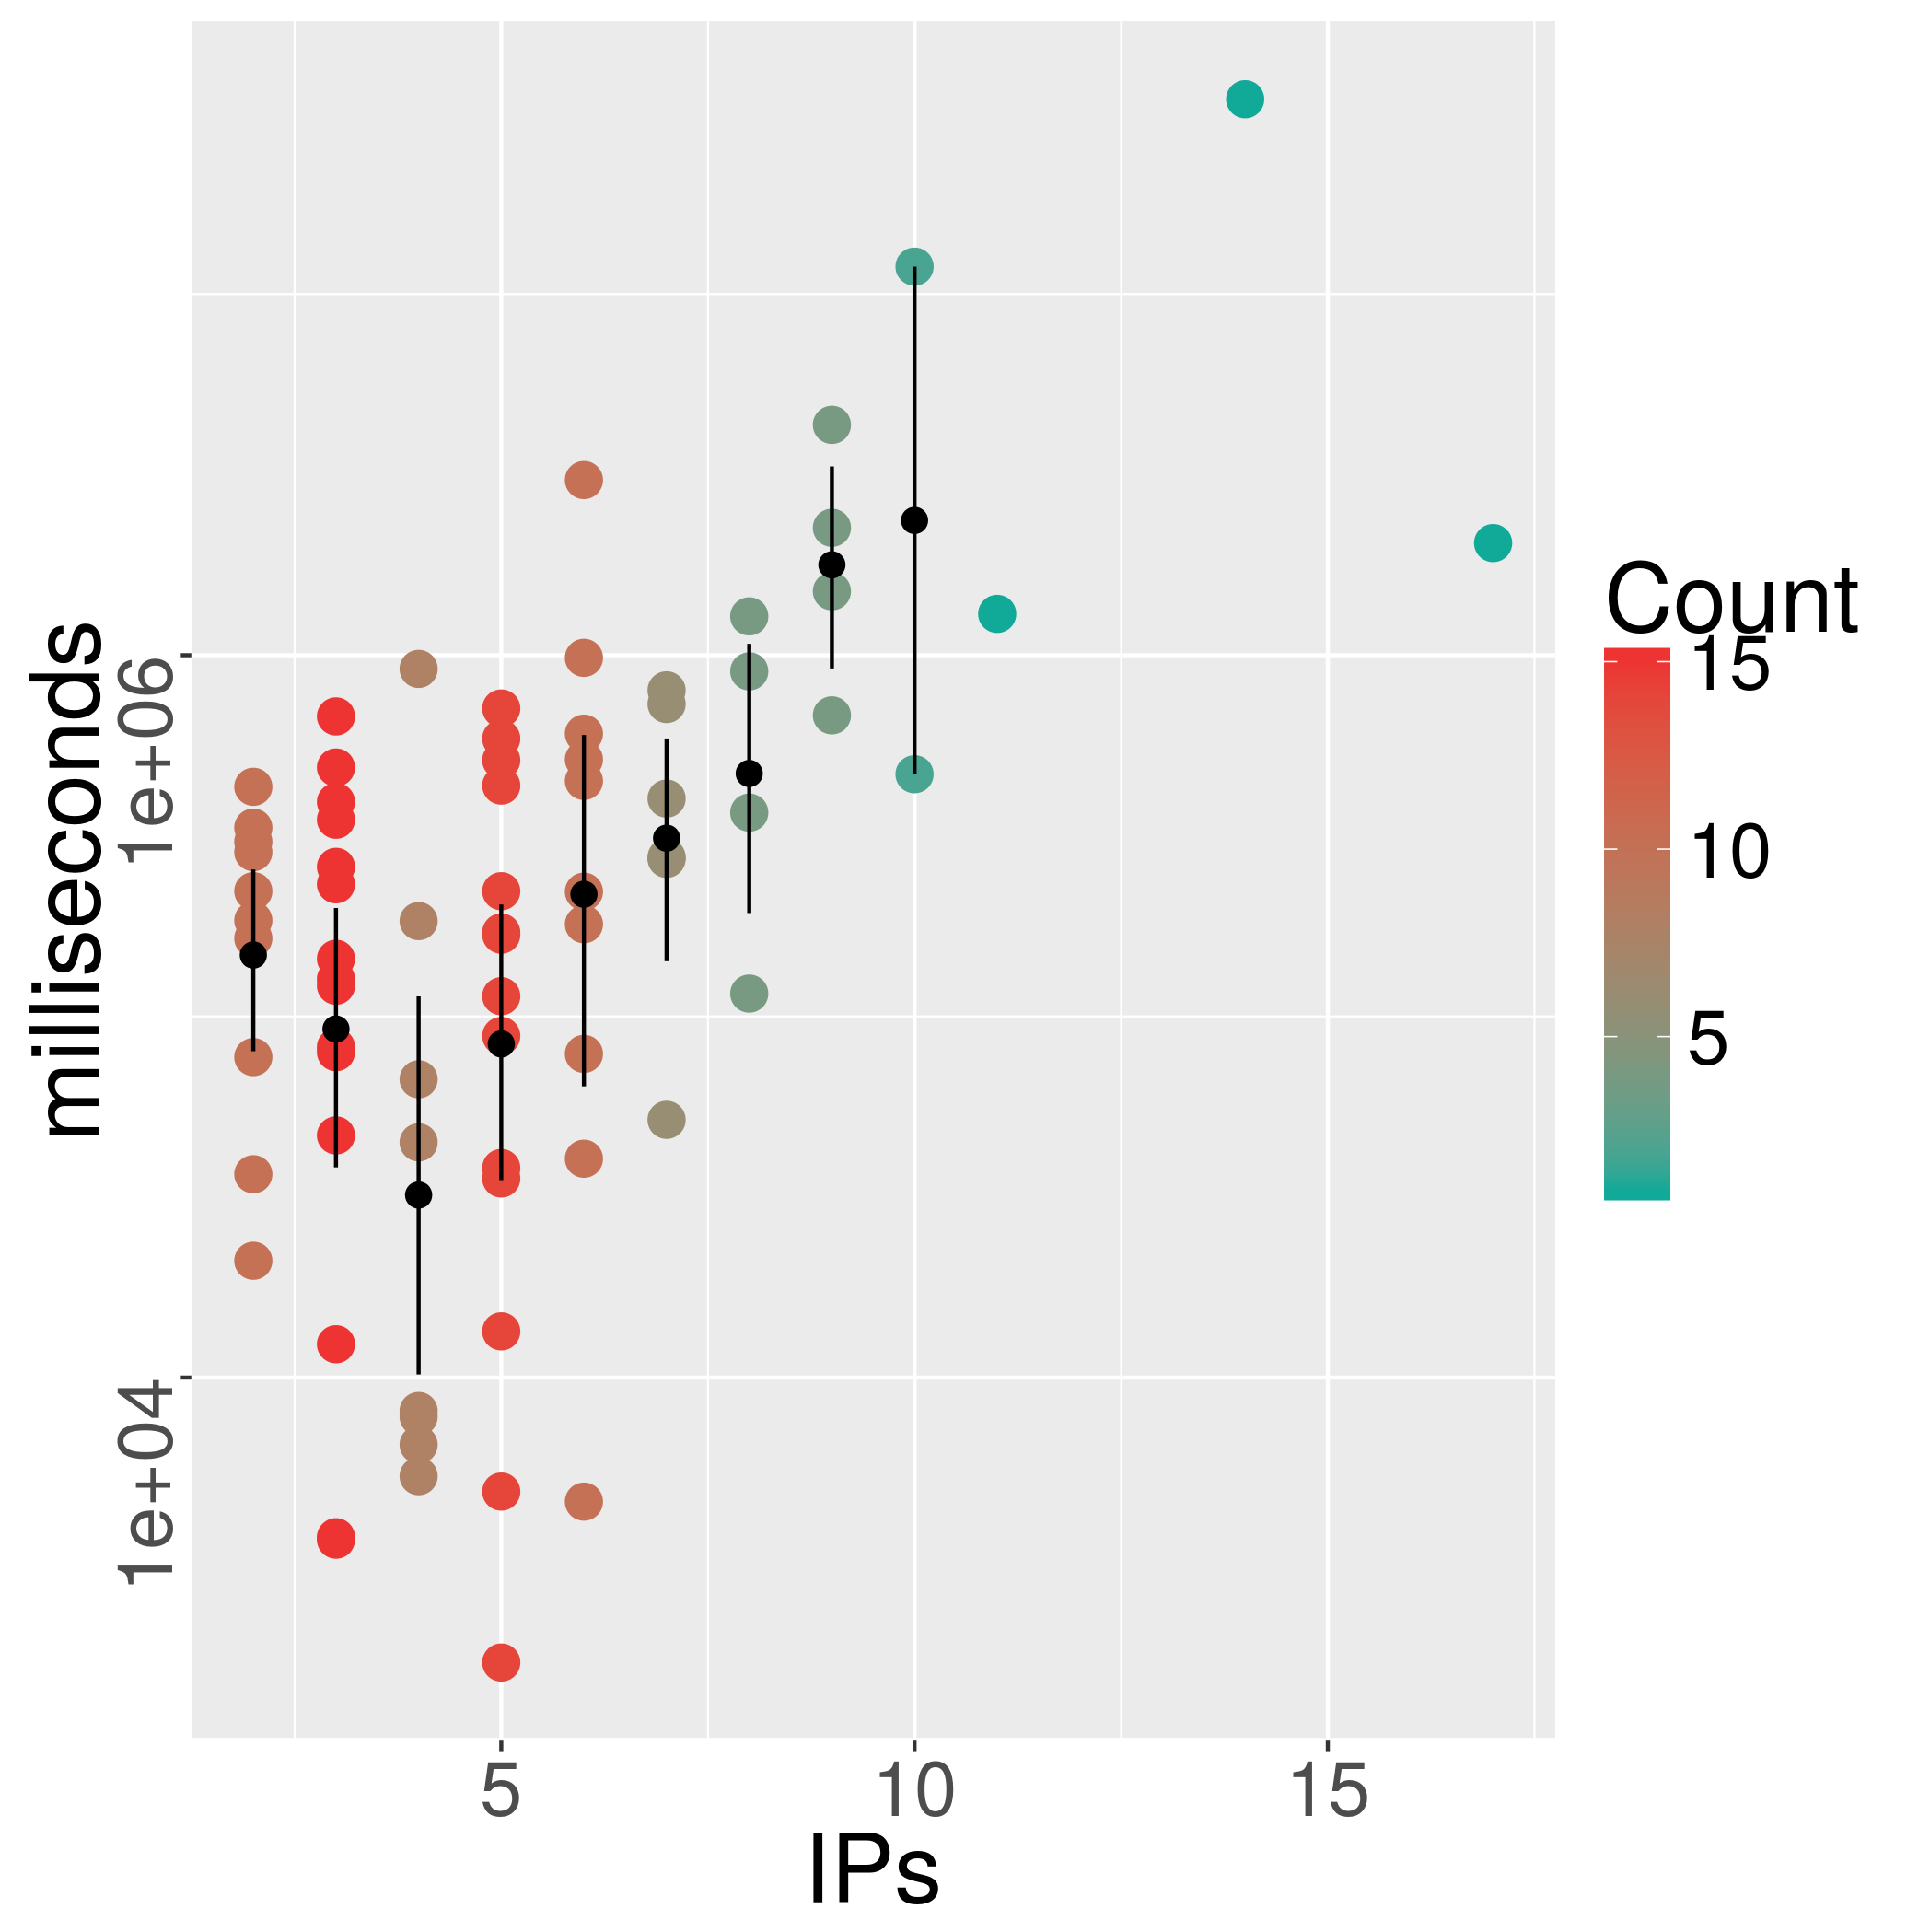
\includegraphics[width=0.32\linewidth]{time-vs-ips-alife-128.png}
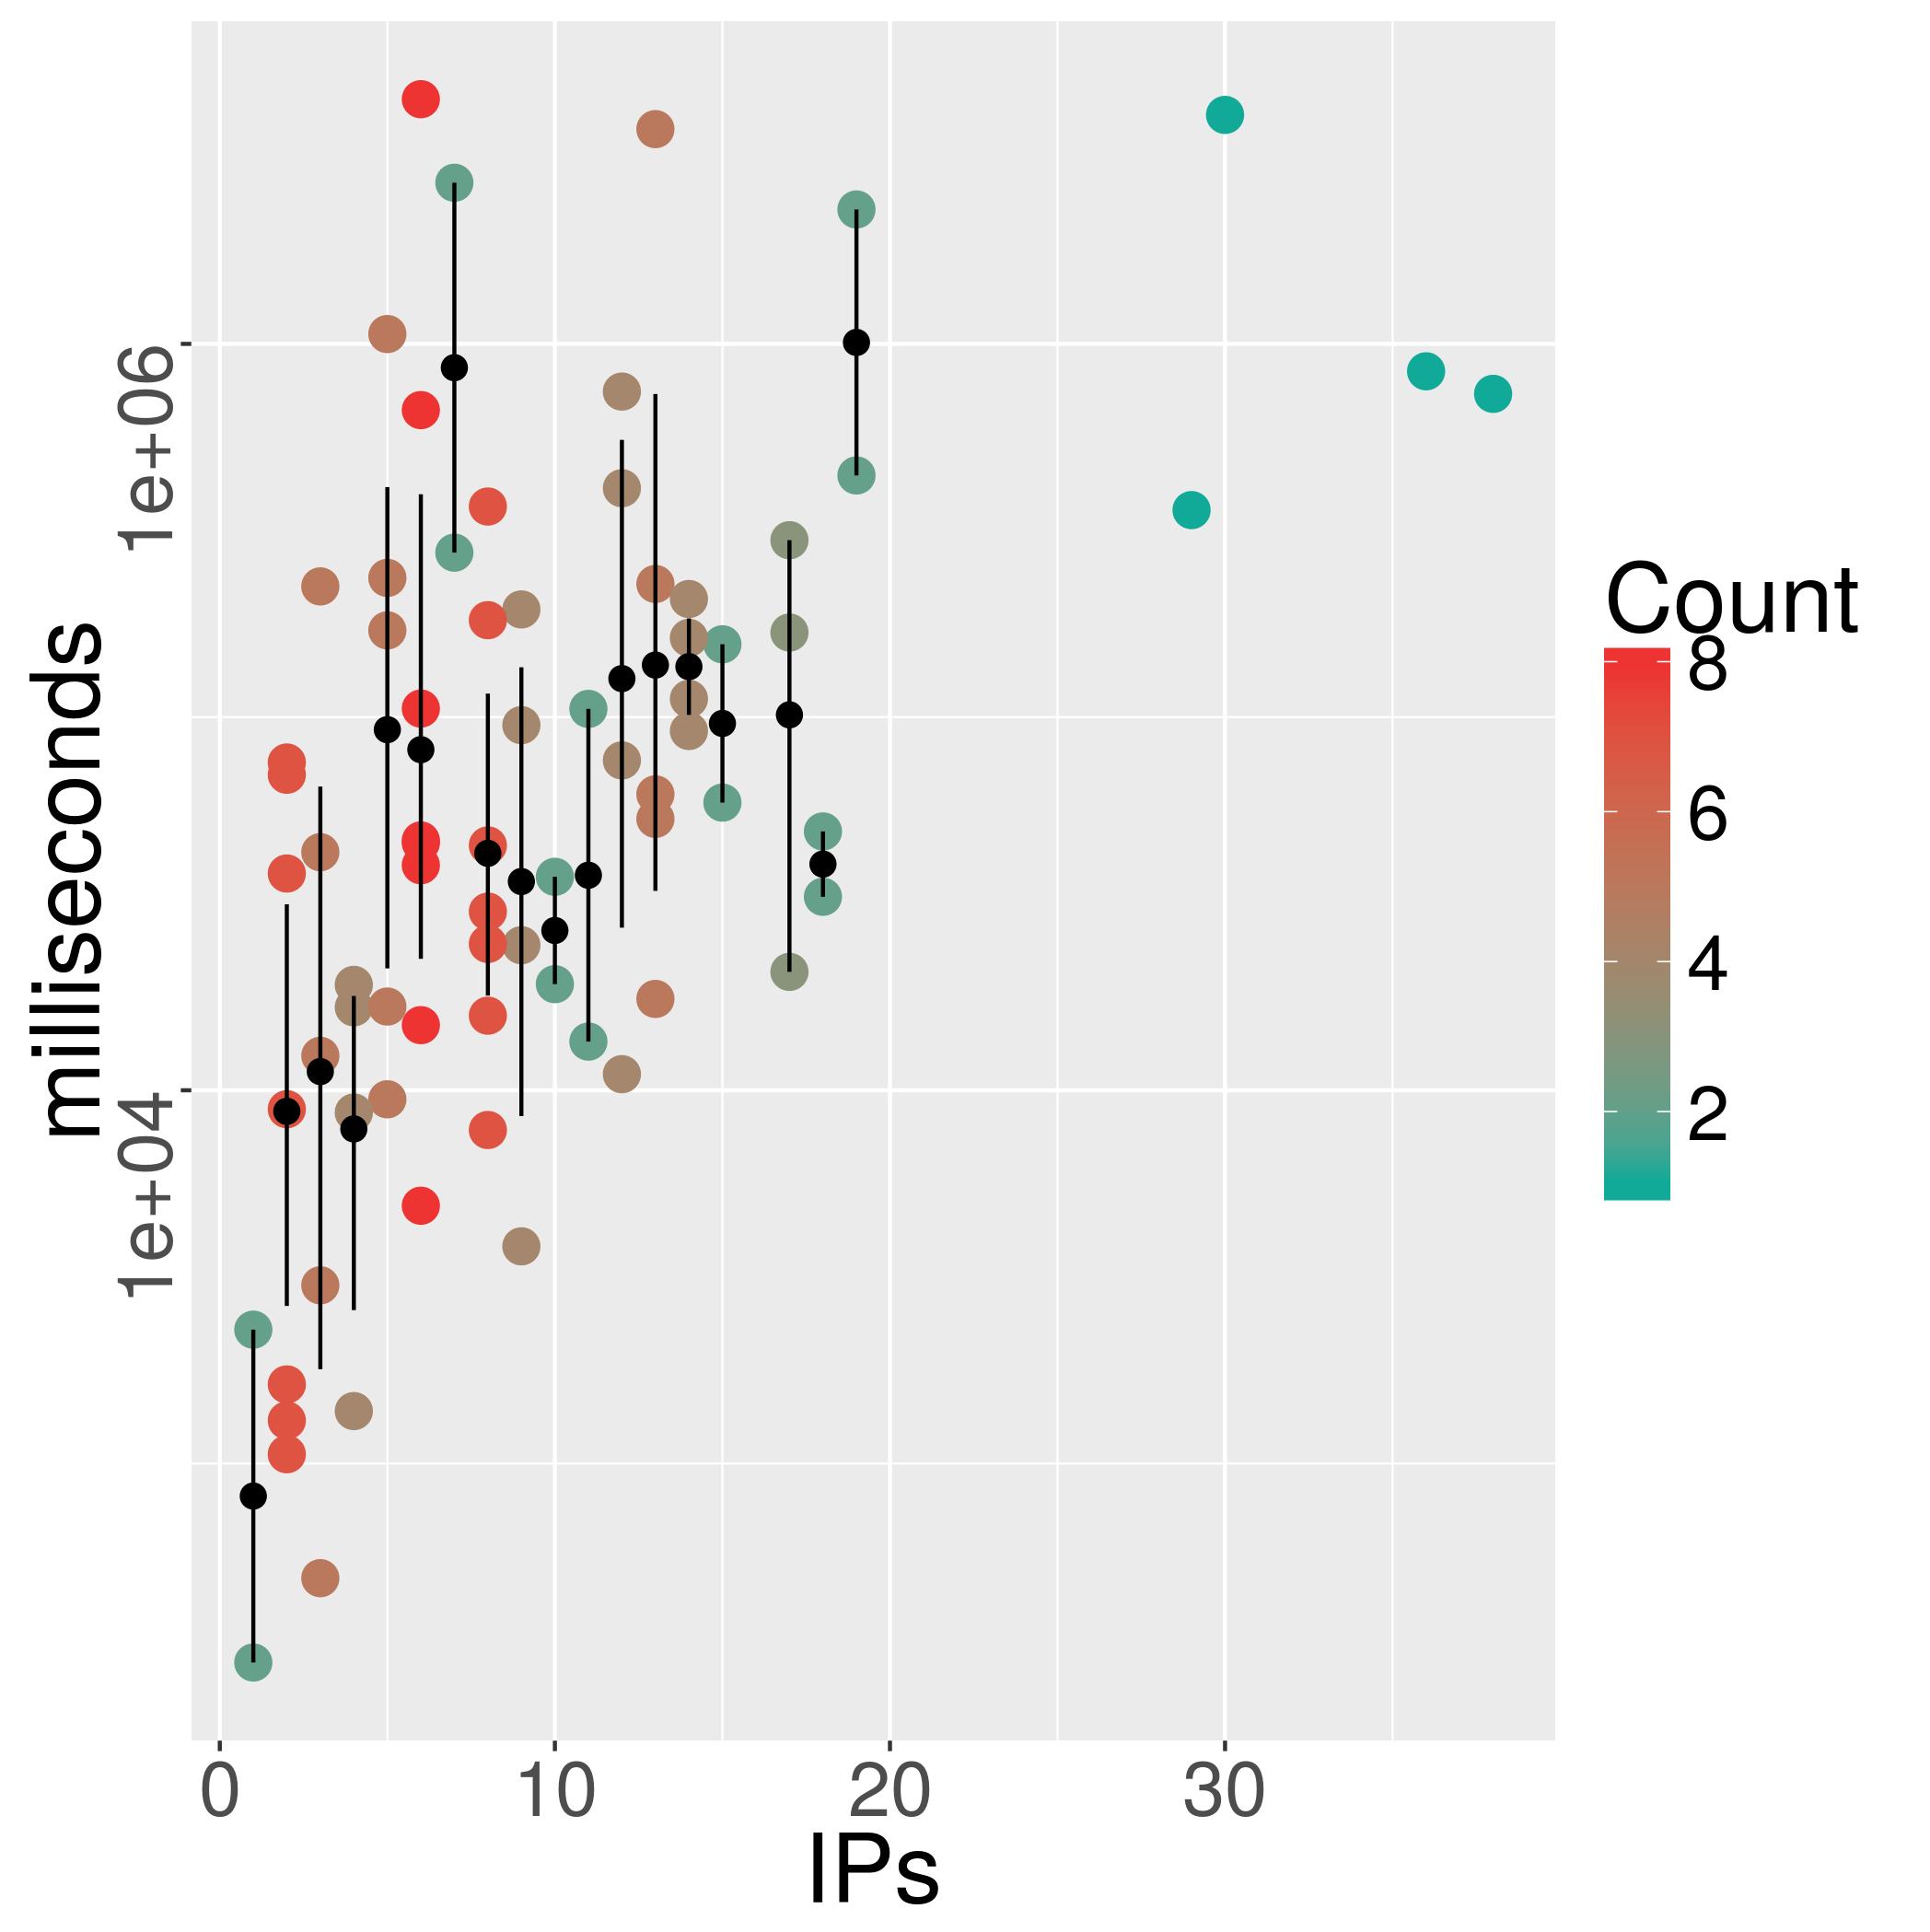
\includegraphics[width=0.32\linewidth]{time-vs-ips-alife-64.png}
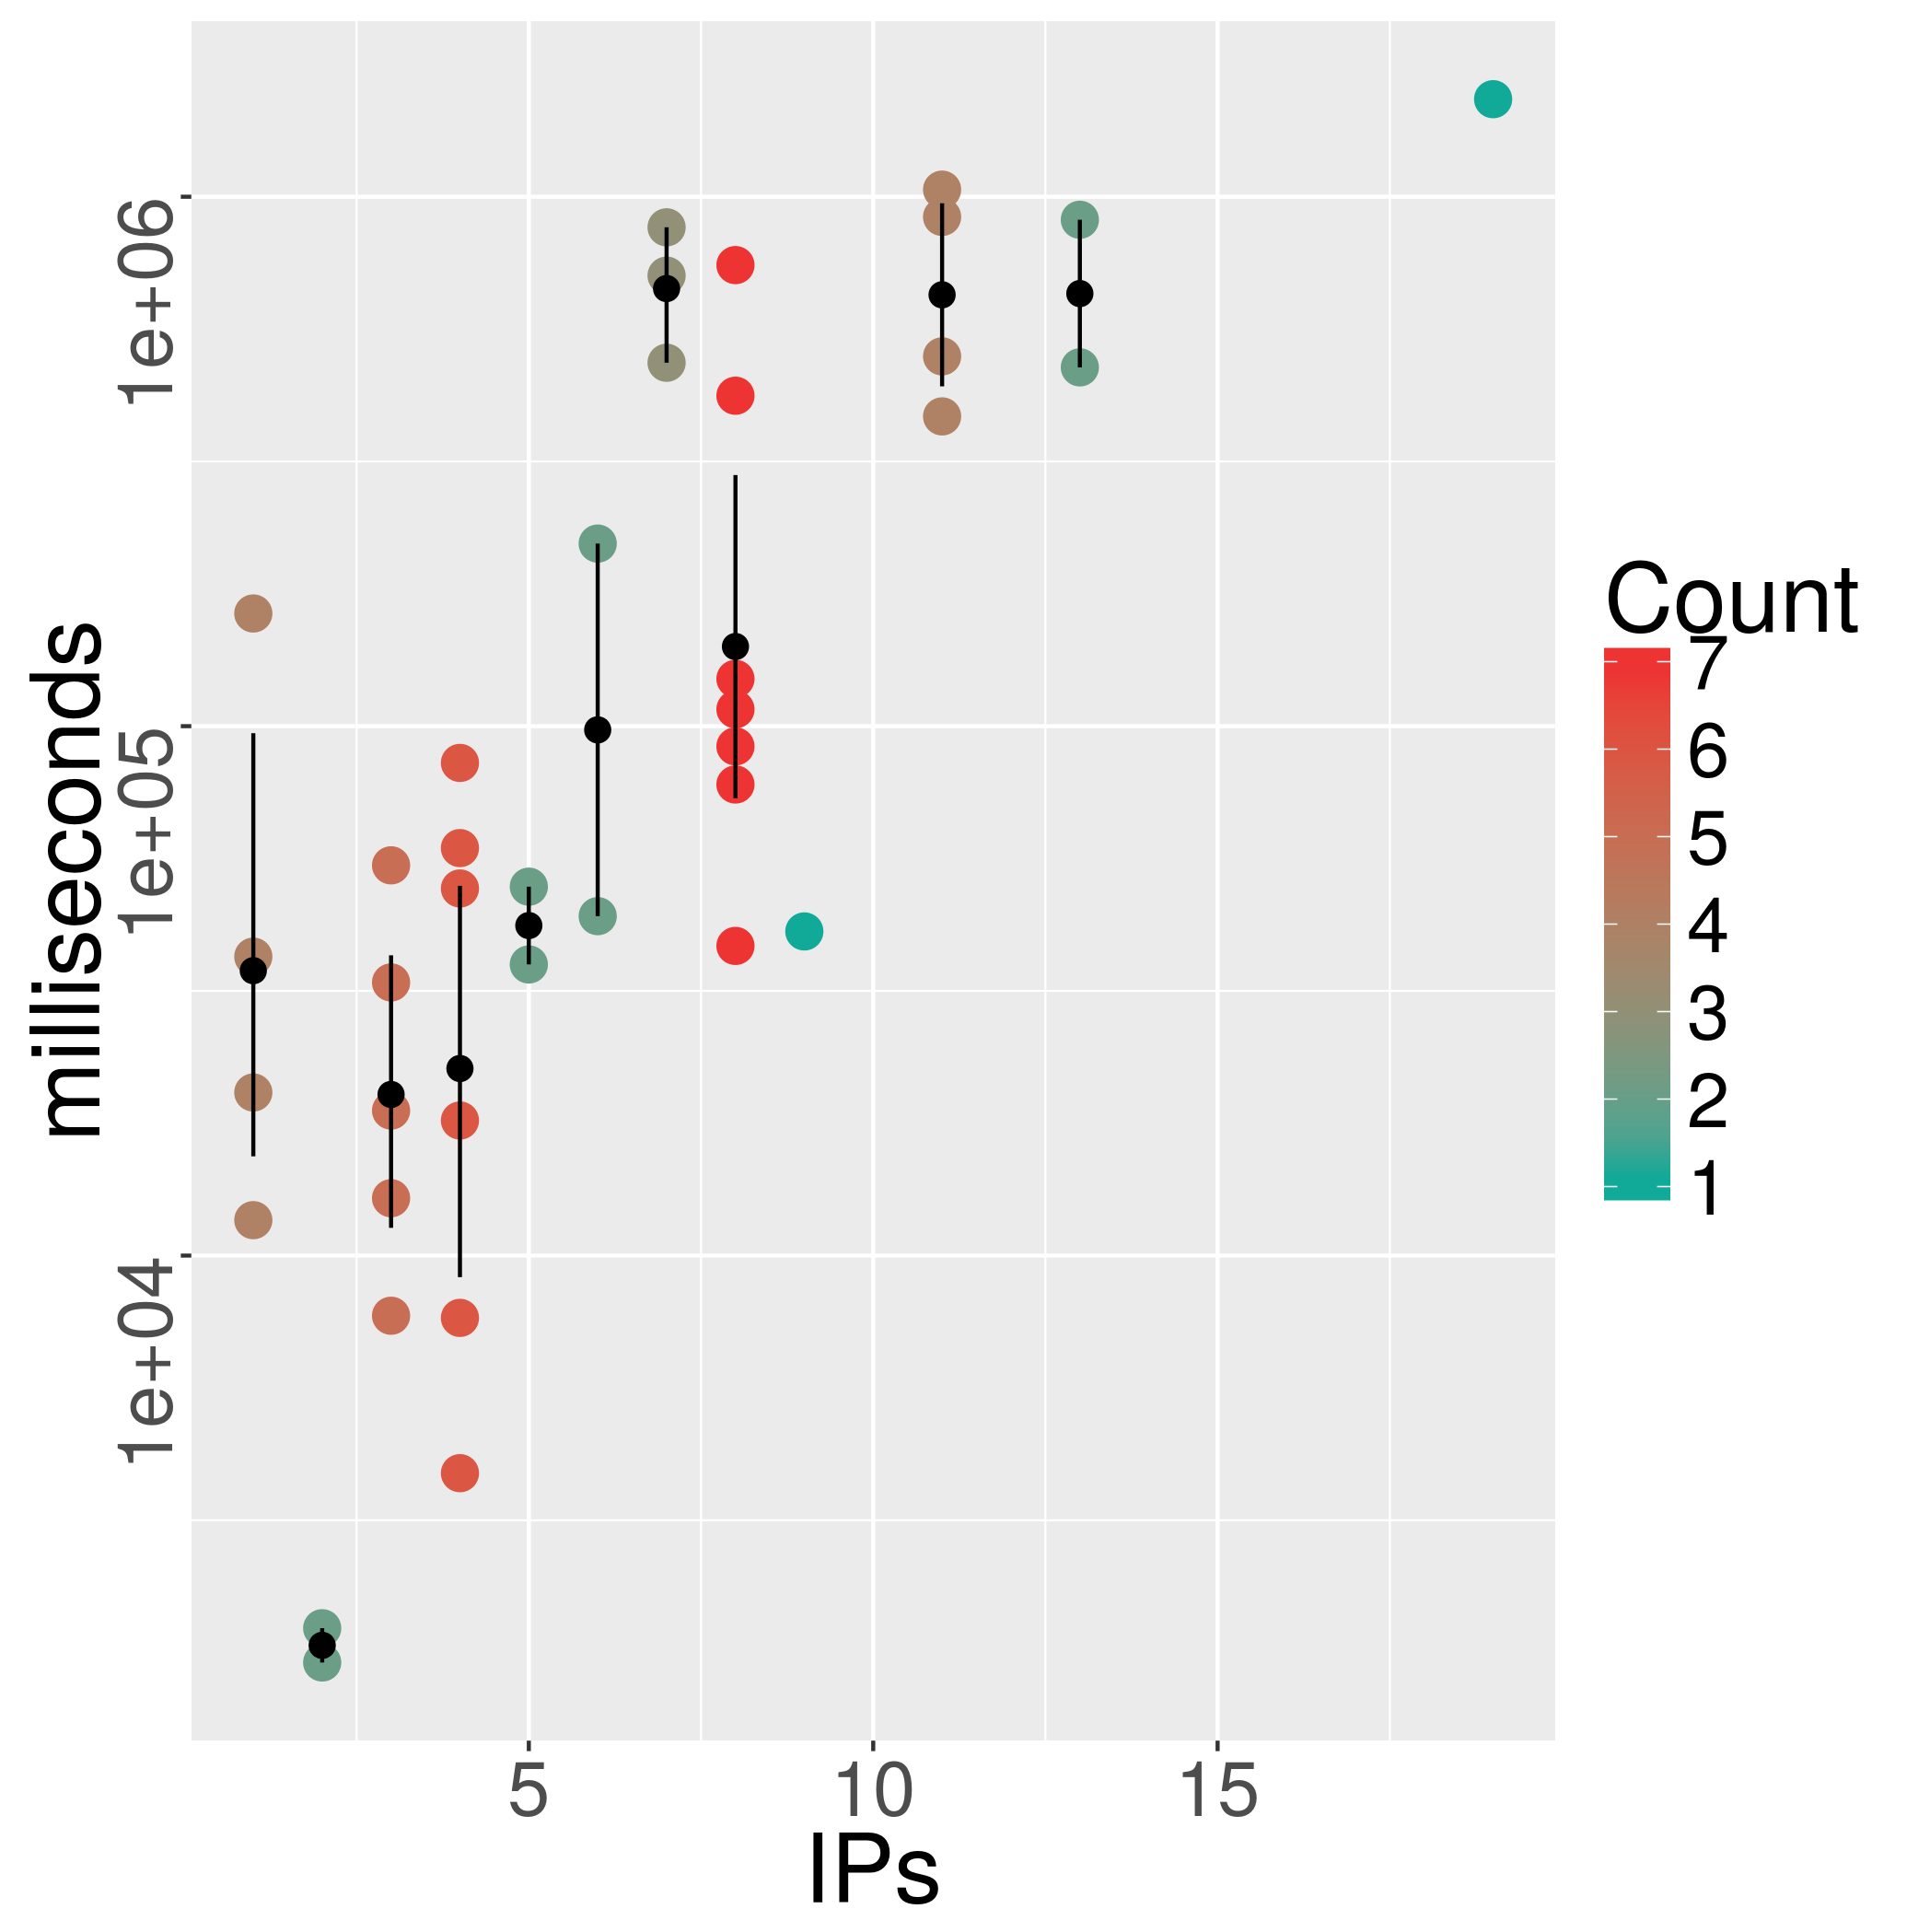
\includegraphics[width=0.32\linewidth]{time-vs-ips-alife-32.png}
\caption{Duration of experiments vs. number of different IPs (nodes)
  participating in it, with averages and standard deviation shown as
  red dots; in the case there is a single red dot, there was a single
  experiment in which many computers participated (for instance, 16
  computers in the experiment in the far left or 29 in the middle
  one). 
Shades of blue indicate how many experiments included that many unique IPs,
so lighter shade for a column of dots indicates that a particular number
of computers happened less frequently, while darker shadow means more frequency. 
From left to right and top to bottom experiments 4/4, 4/24 and 7/31,
followed by experiments with 50 traps, cache=128, 64, 32.}
\label{fig:duration}
\end{figure}
%
We will have to analyze experimental data a bit further to find out why
this happens and also if there are some patterns in the three sets of
experiments. An interesting question to ask, for instance, is if
by adding more computers makes the experiment take less. In fact, as
shown in Figure \ref{fig:duration}, the {\em addition} of more computers does
not seem to contribute to decreasing the time needed to finish the
experiment. However, the cause-effect relationship is not clear at
all. It might be the opposite: since experiments take longer to finish
and might in fact be abandoned with no one contributing for some time,
the probability of someone new joining them is higher. In fact,
with experiments taking a few seconds and due to the way the
experiments are announced, it is quite difficult that several
volunteers join in in such a short period of time, even more if we take
into account that volunteers are not {\em carried over} from previous
experiments. 
%
\begin{figure}[!htb]
\centering
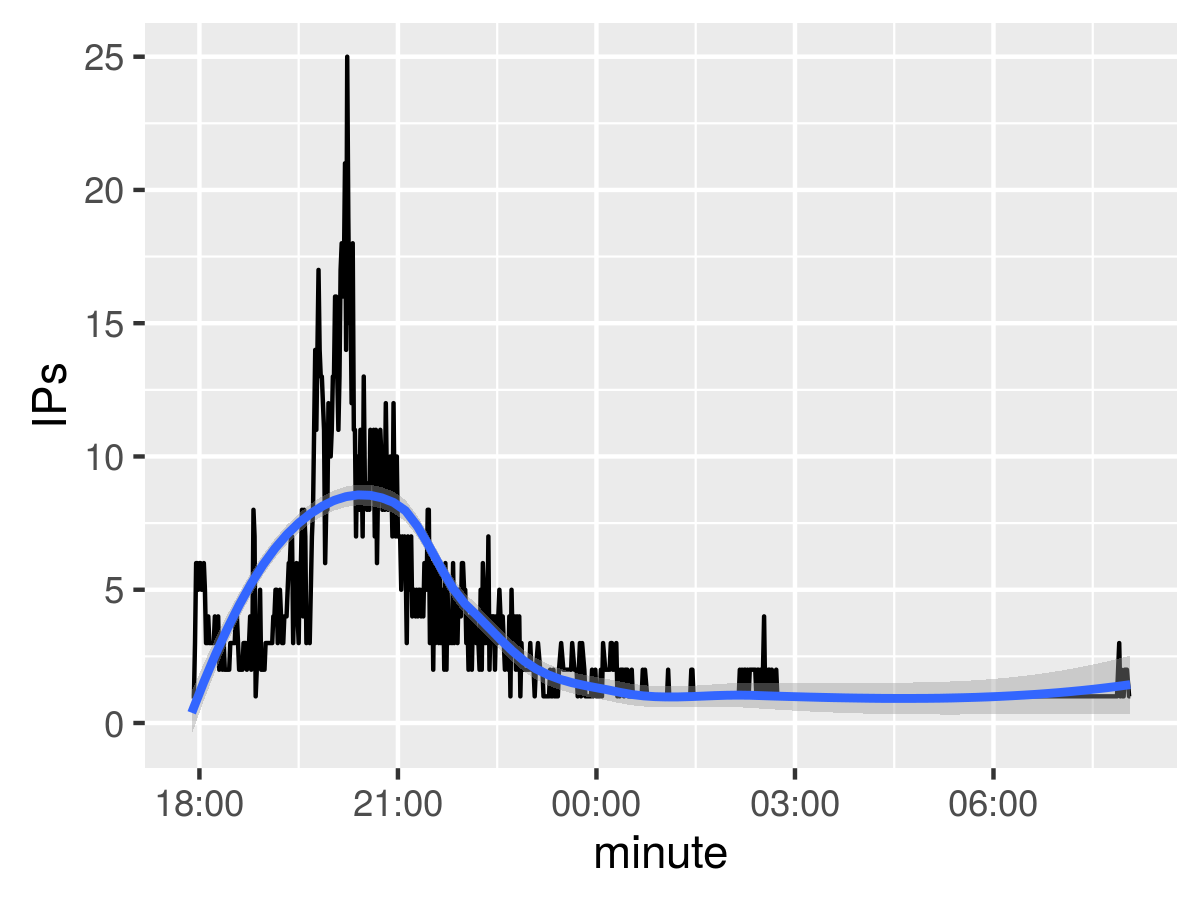
\includegraphics[width=0.95\linewidth]{ips-per-minute-cache=64.png}
\caption{Simultaneous IPs every minute of the experiment with cache =
  64. \label{fig:otisdriftwood}}
\end{figure}


That is why we used a more difficult problem in the second batch of
experiments, which is shown in bottom row of Figure
\ref{fig:duration}. The pattern is remarkably similar, showing a
positive correlation between the time for solving the problem and the
number of computers, at least for cache sizes 128 and 64. However, it
is interesting to observe that, for cache=32, the time needed to find
the solution decreases from one to approximately 4-5 nodes, to then
increase for a higher number of participating computers, distinguished
by IP. The green dot at the bottom is probably and outlier that we
will try to explain later on. This leads us to conclude that a better
amount of computers might contribute to speed up the solution, if the
time the experiment ideally takes is sufficient, that is, of the order of a
minute, and enough volunteers concur simultaneously. This is also
observed, not so clearly, in the case of cache=64, with an interval of
around 10 IPs obtaining less time than experiments with less or more
IPs, and of the same order, between 10 and 100 seconds. If we look at
the graph that shows the number of IPs or volunteers per minute for
this experiment, shown in Figure \ref{fig:otisdriftwood}, we see that
there are peaks of more than 25 volunteers, and a period of several
hours with a minimum of 6 computers and peaks of more than 10. The
long period after midnight where there is a single volunteer left
masks the success achieved during this set of experiments, from which
we draw two lessons: first, you need a social network influencer to
announce your experiments and second, no matter what, do not do any
experiment after midnight. 

\begin{figure}[!htb]
\centering
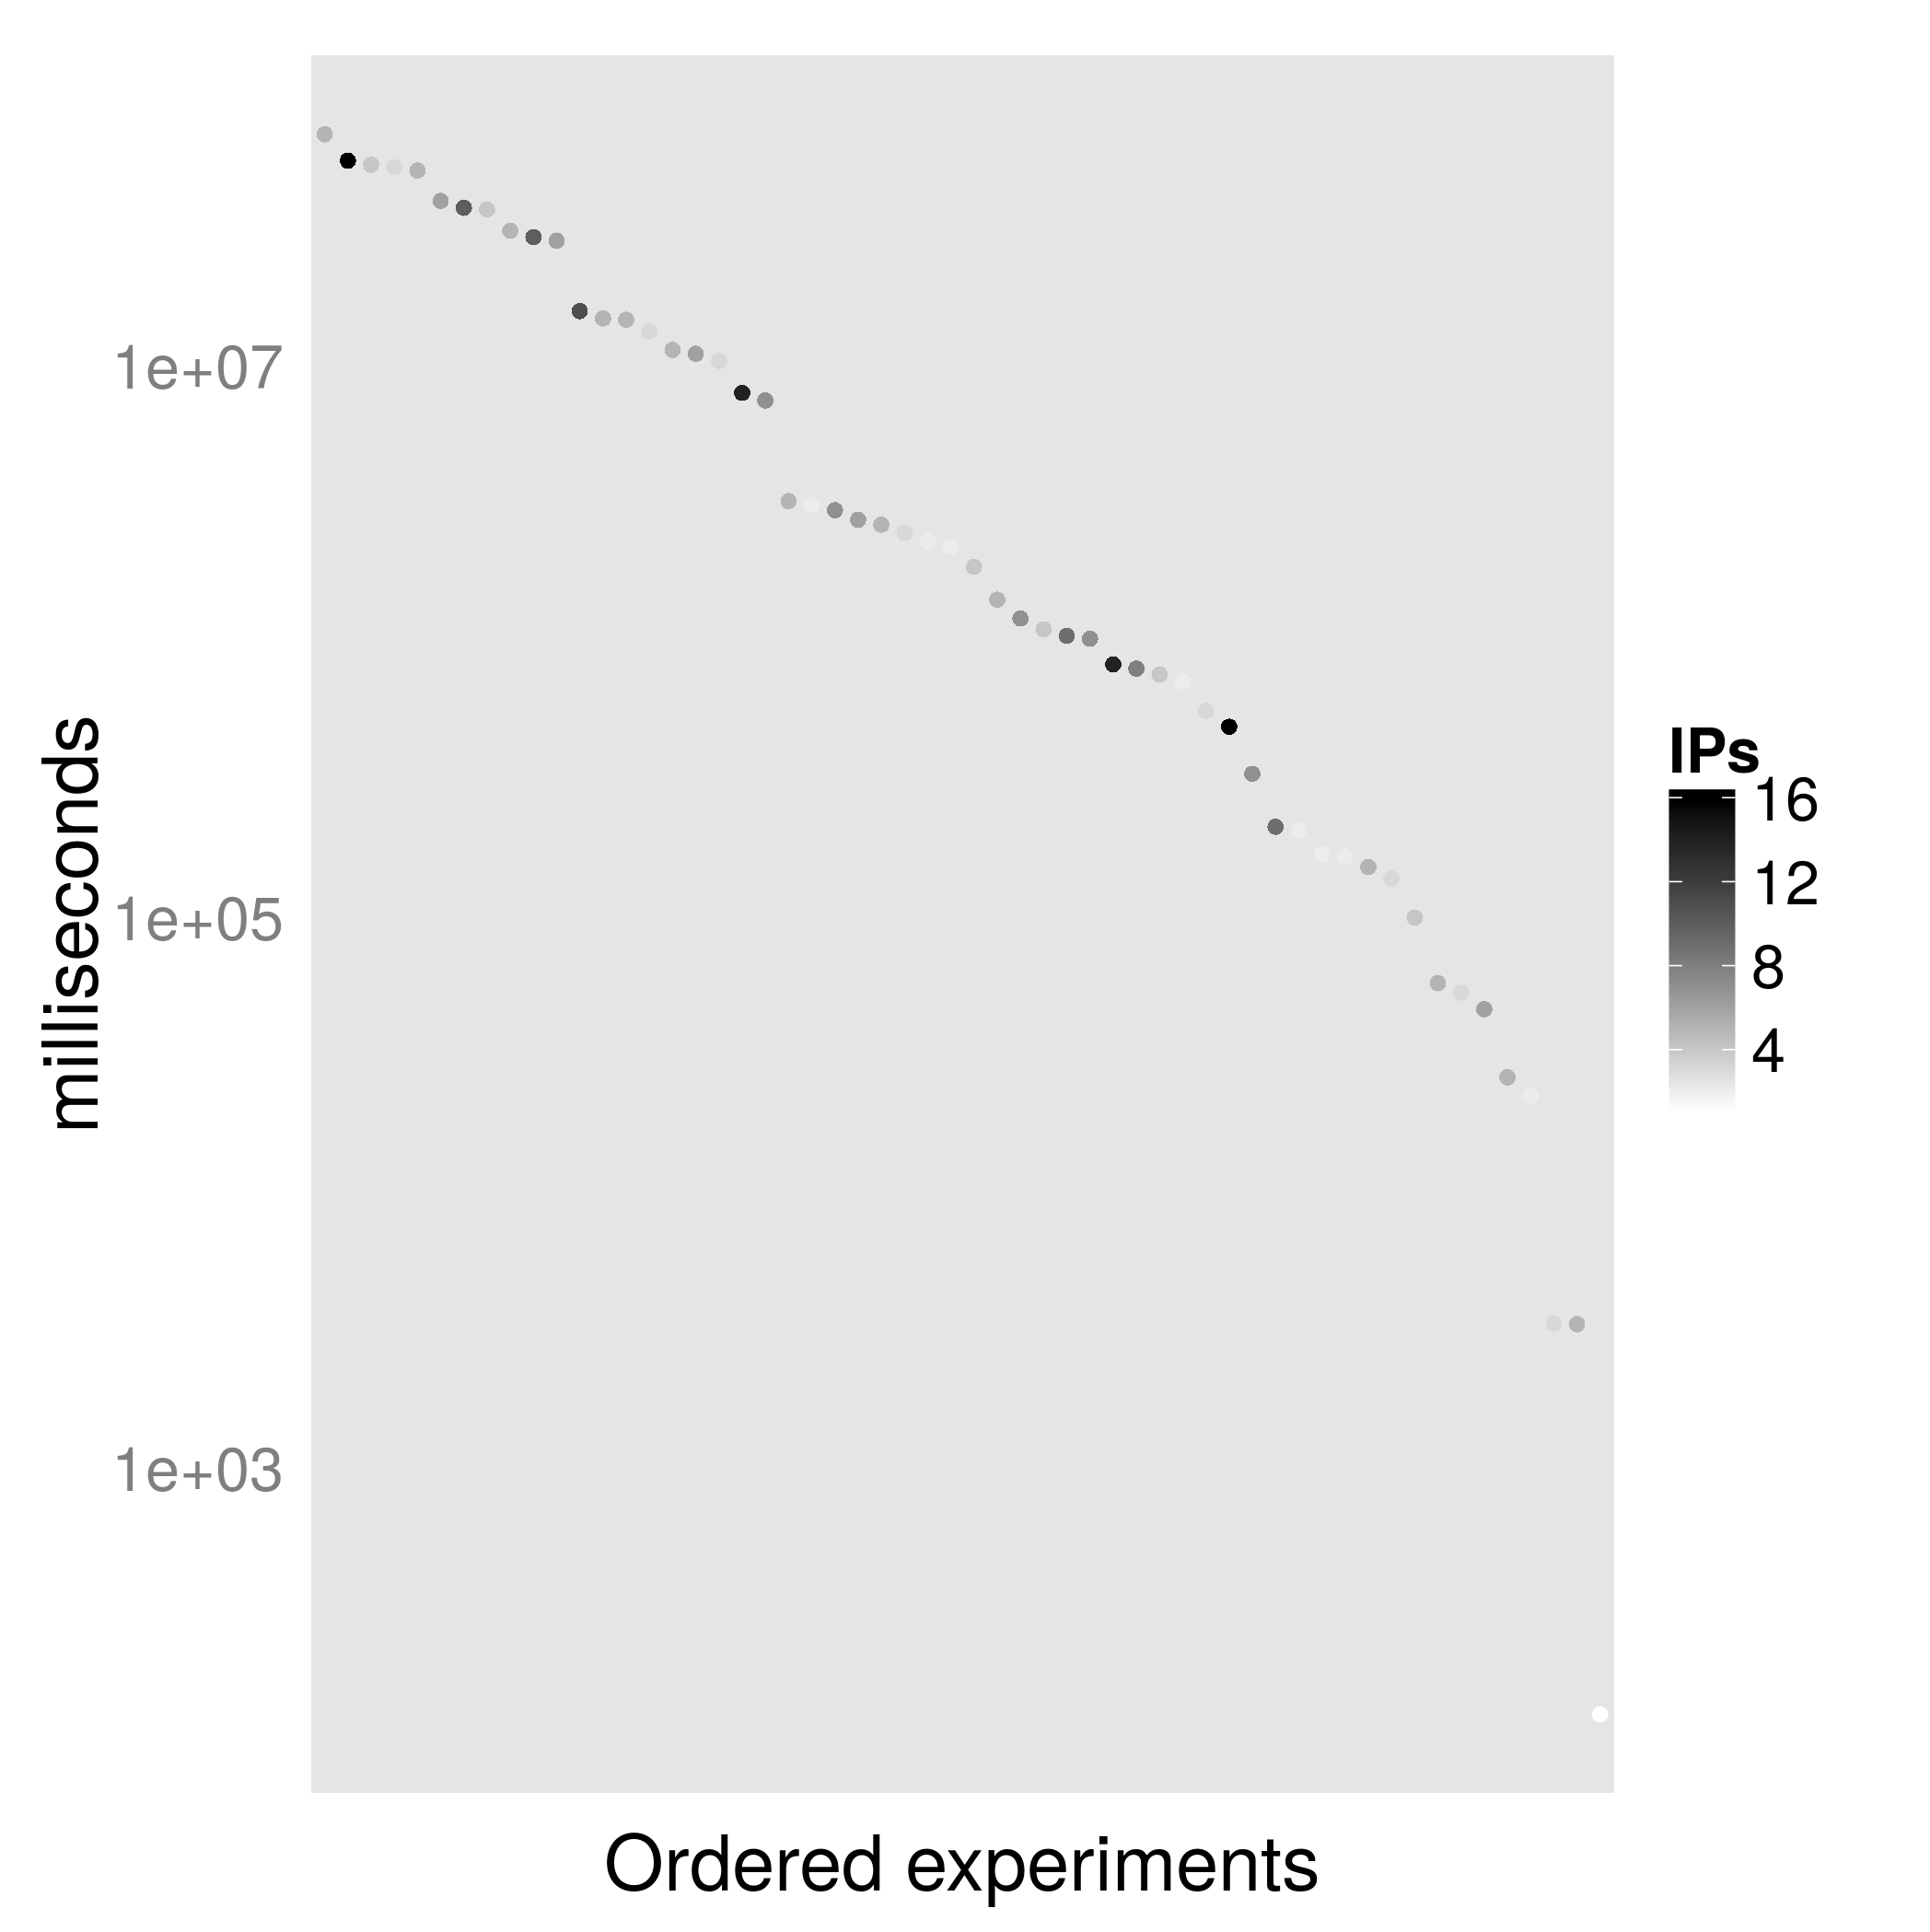
\includegraphics[width=0.32\linewidth]{time-vs-rank-OS-4-4.png}
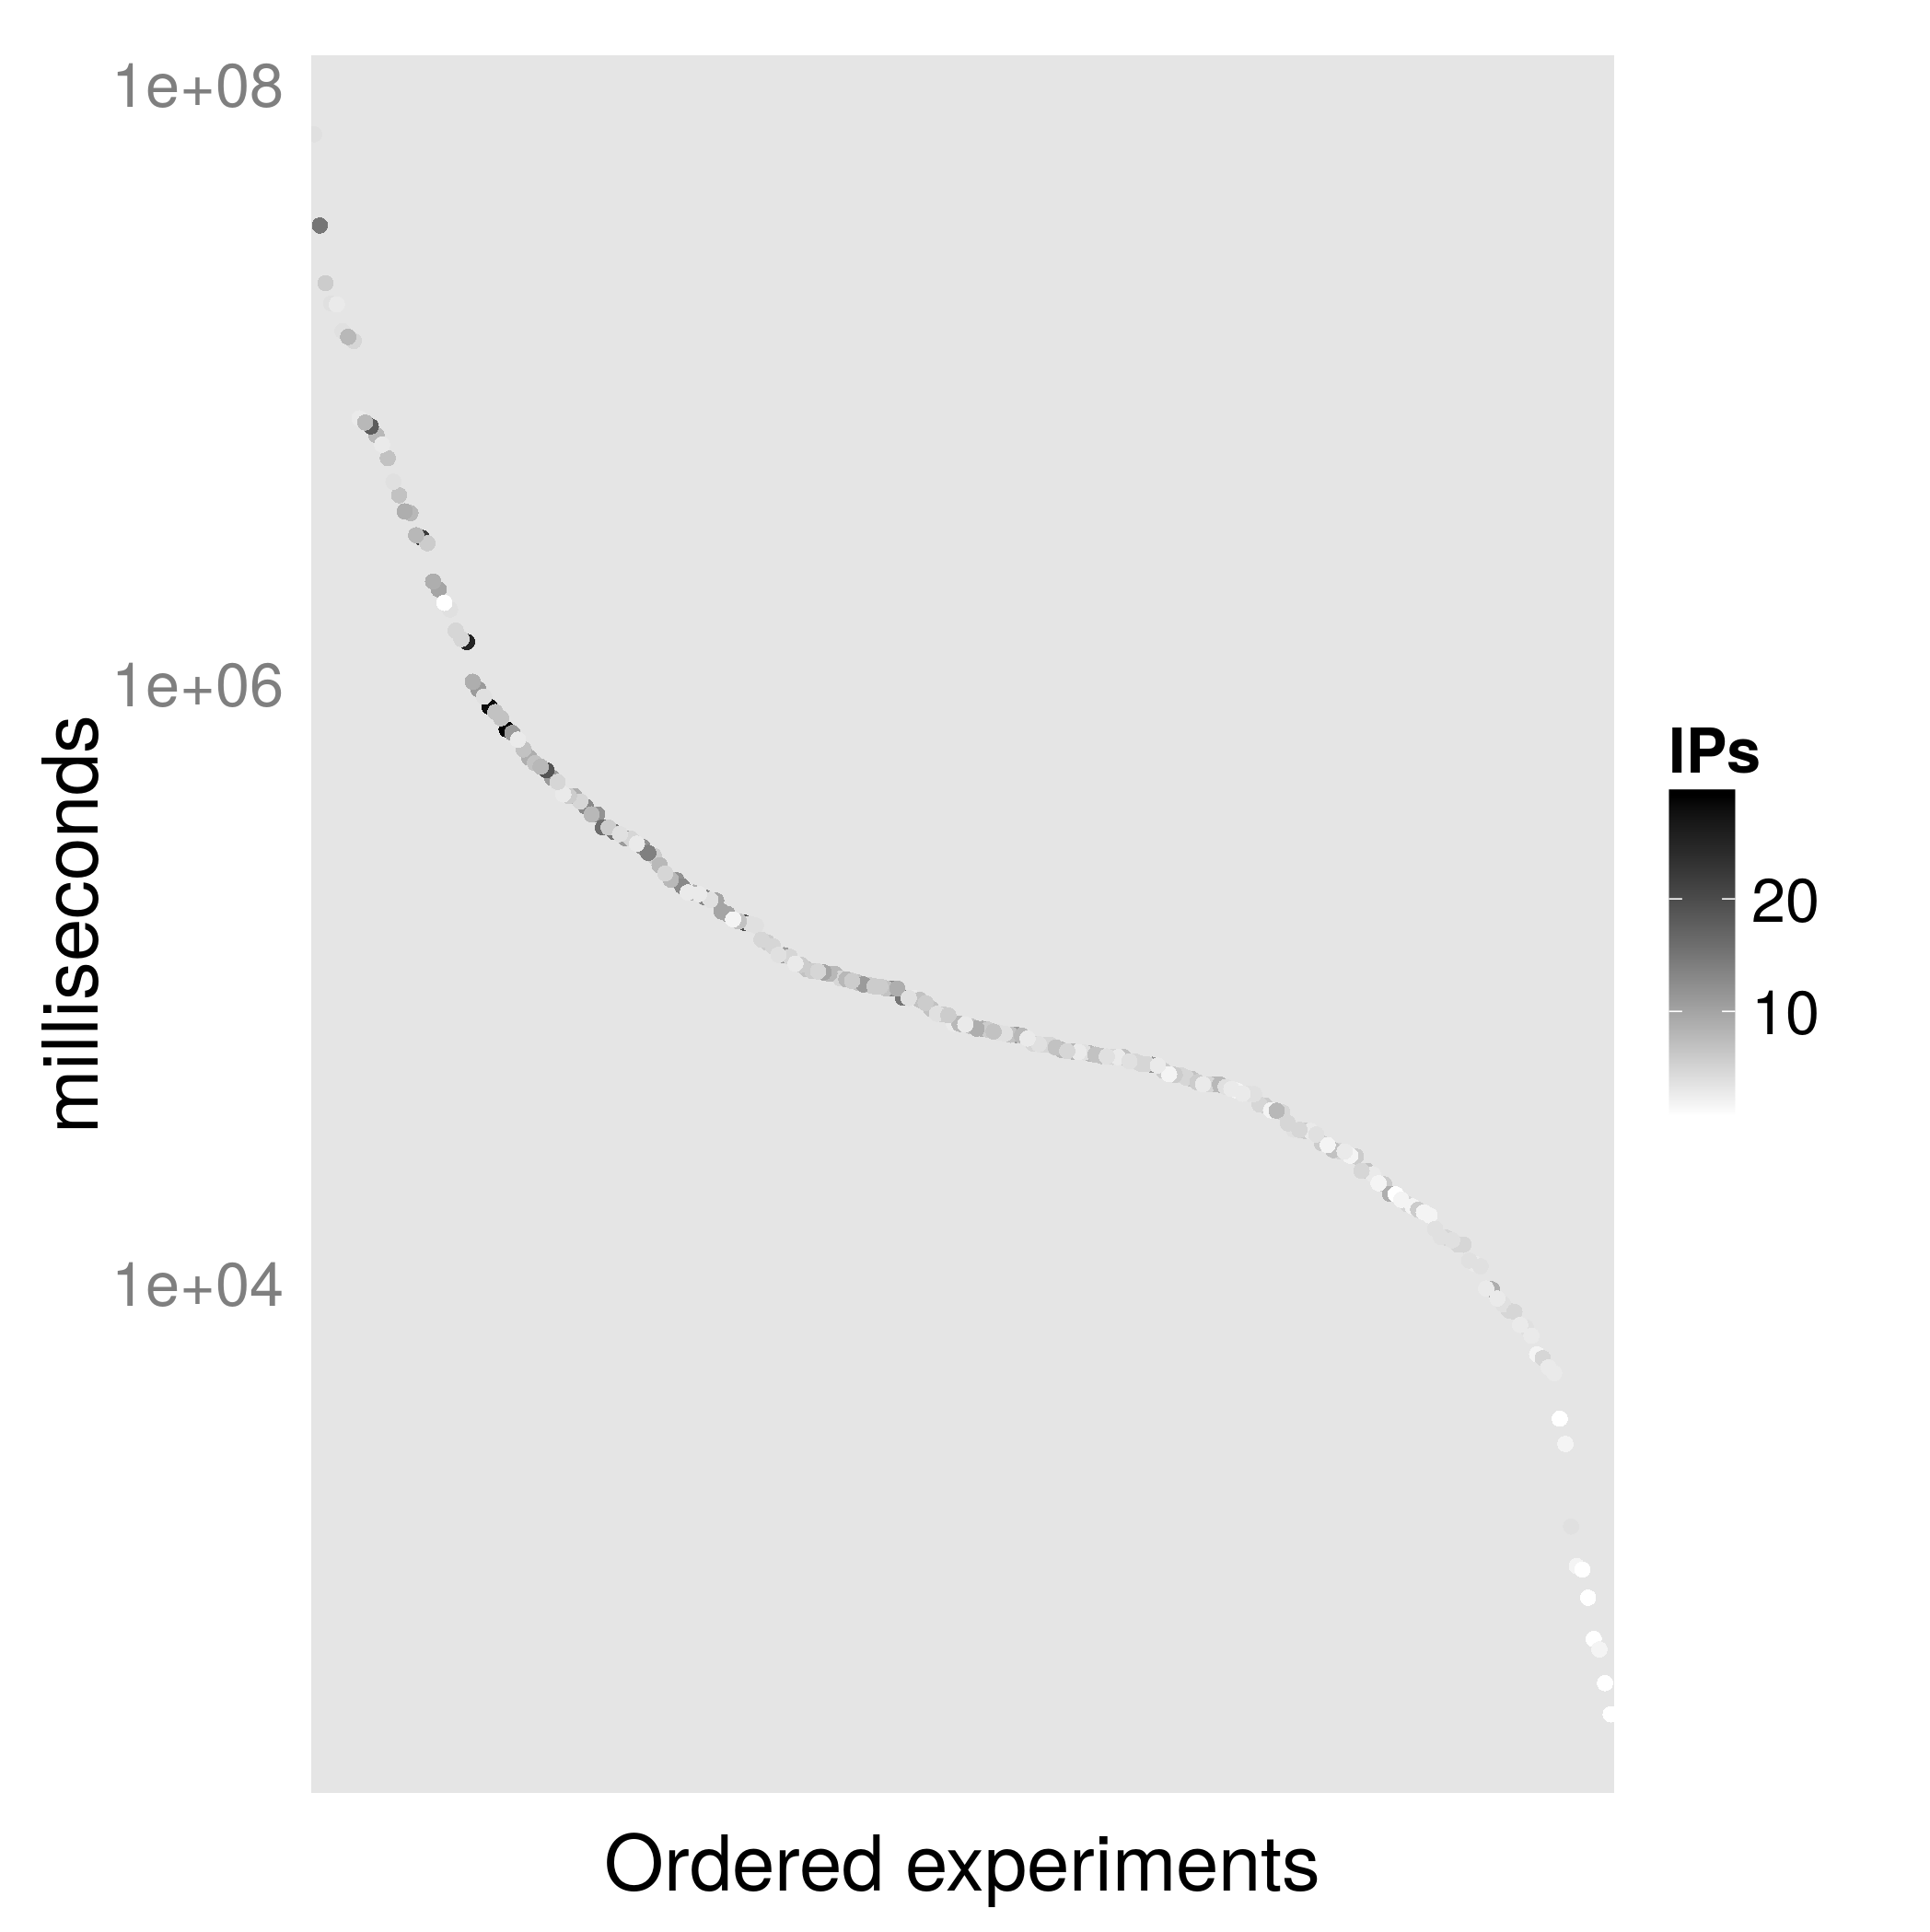
\includegraphics[width=0.32\linewidth]{time-vs-rank-OS-4-24.png}
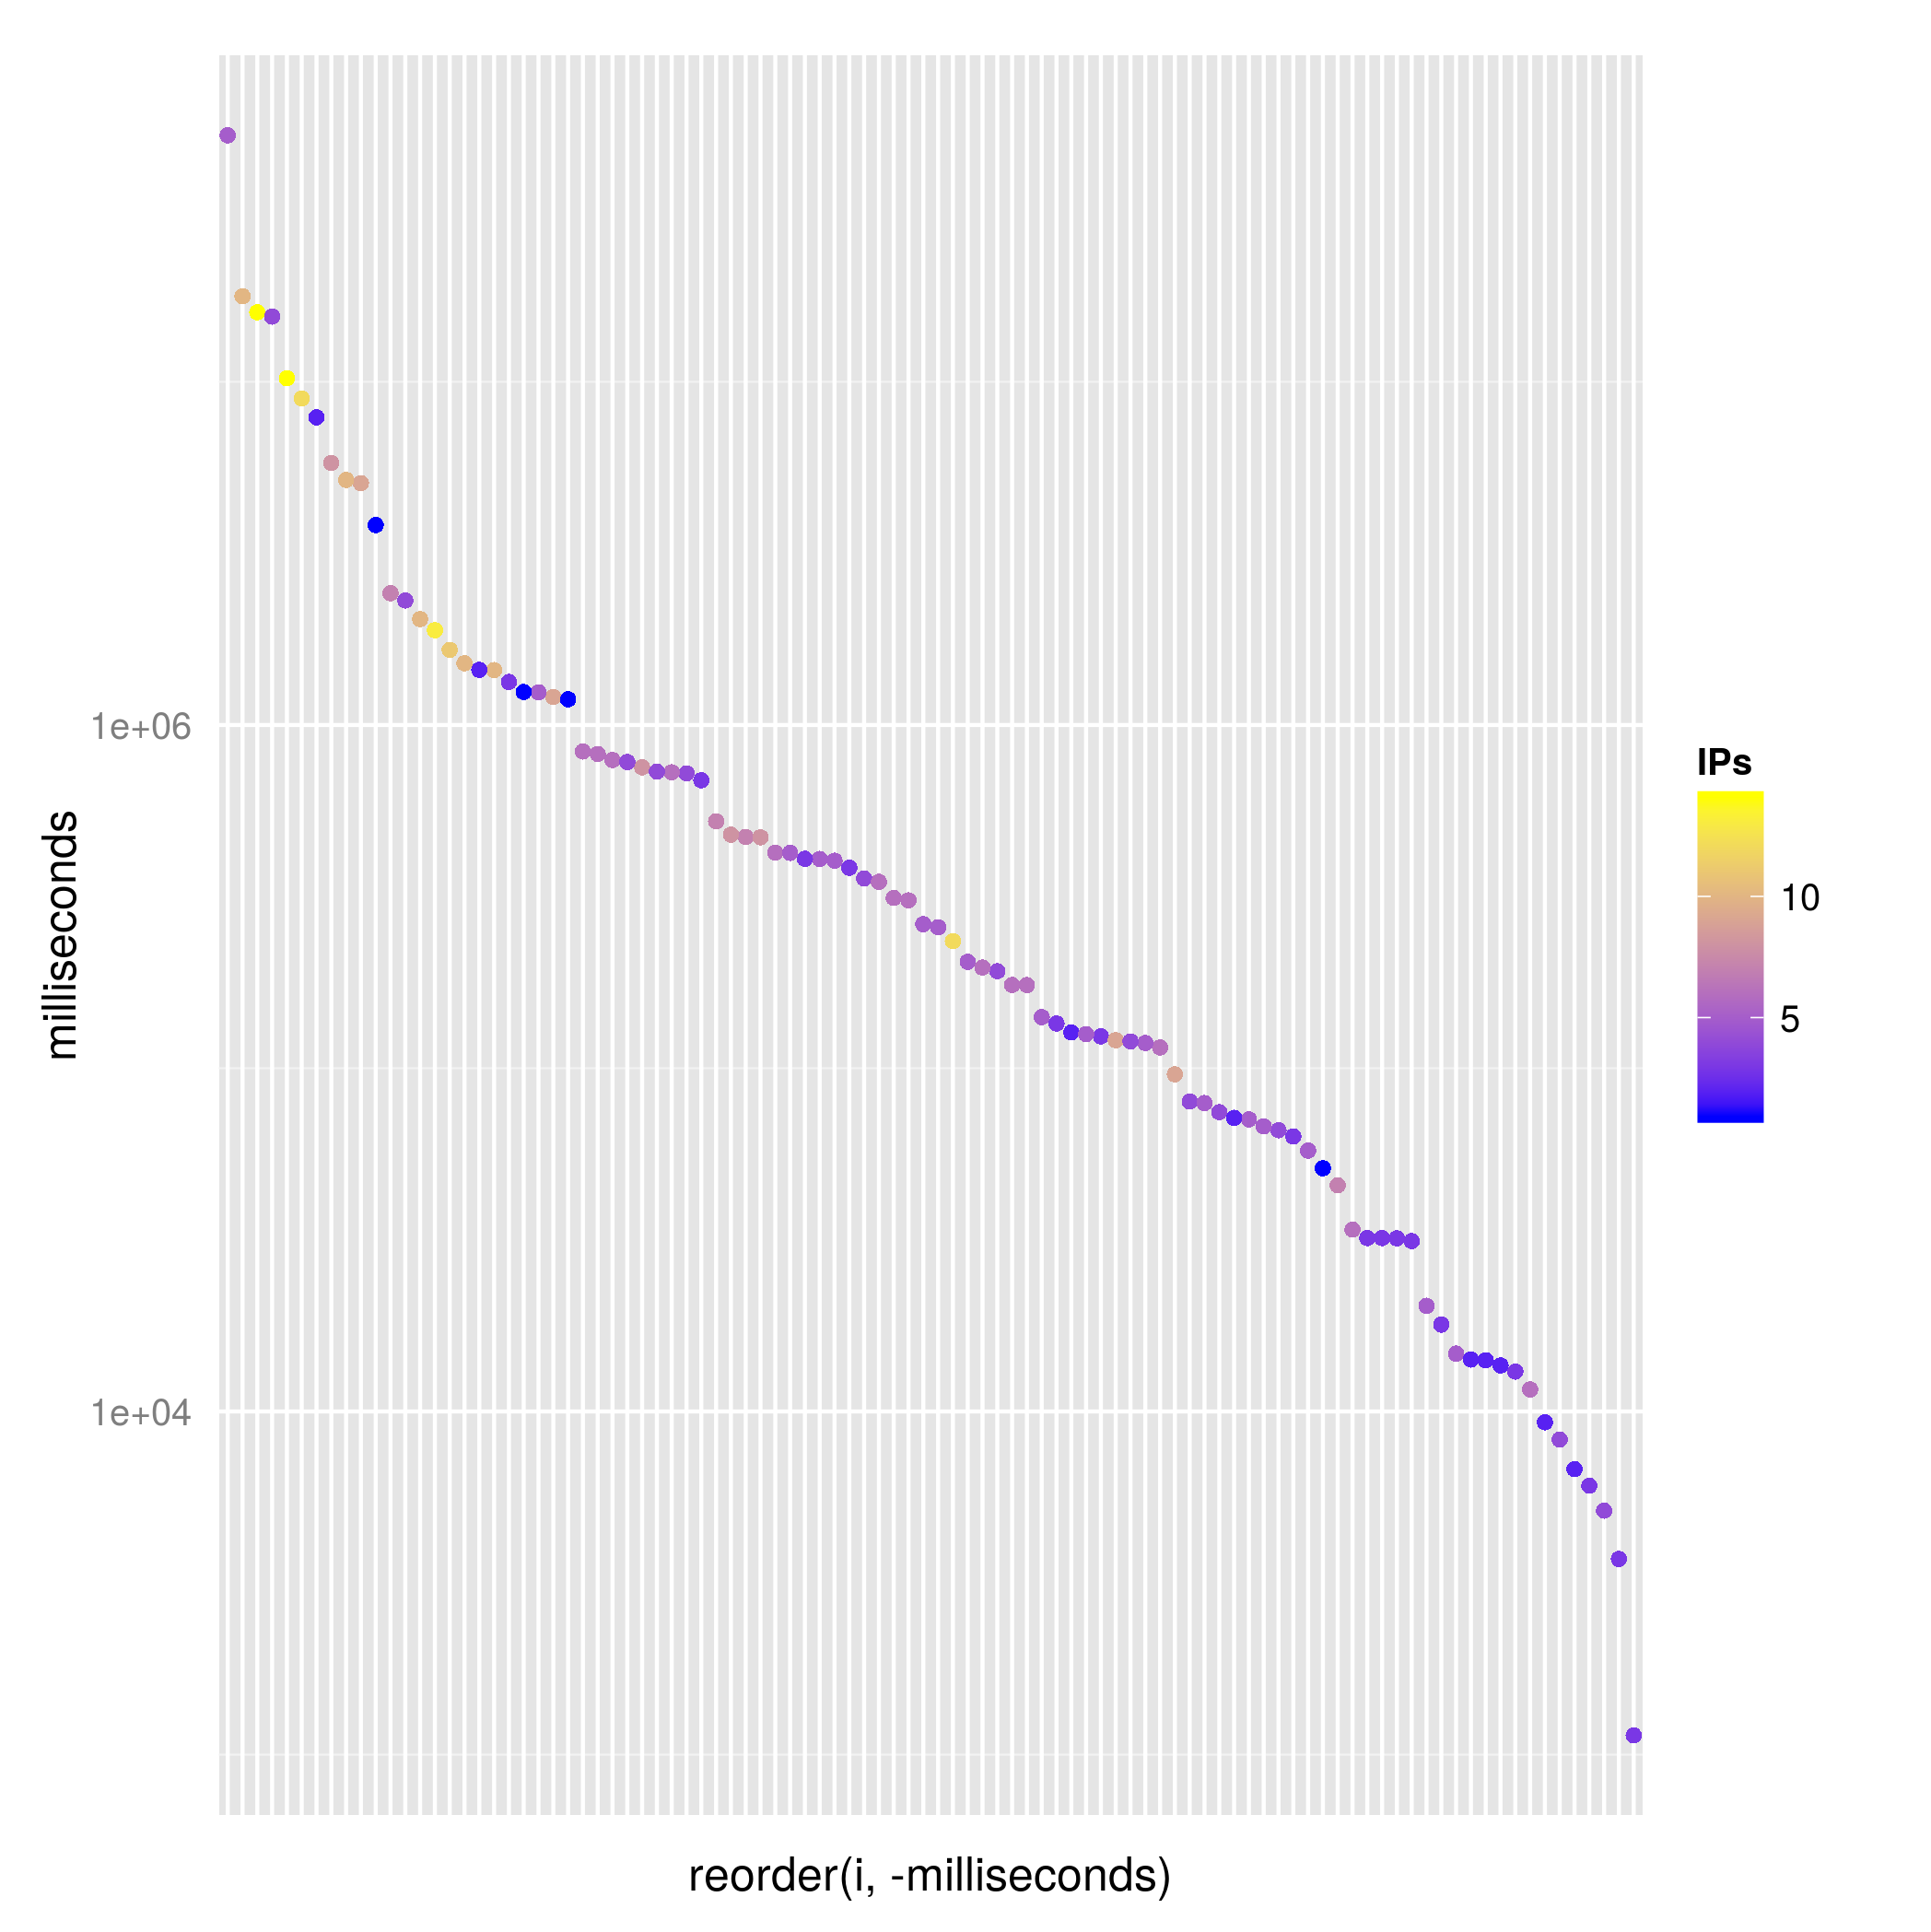
\includegraphics[width=0.32\linewidth]{time-vs-rank-OS-7-31.png}
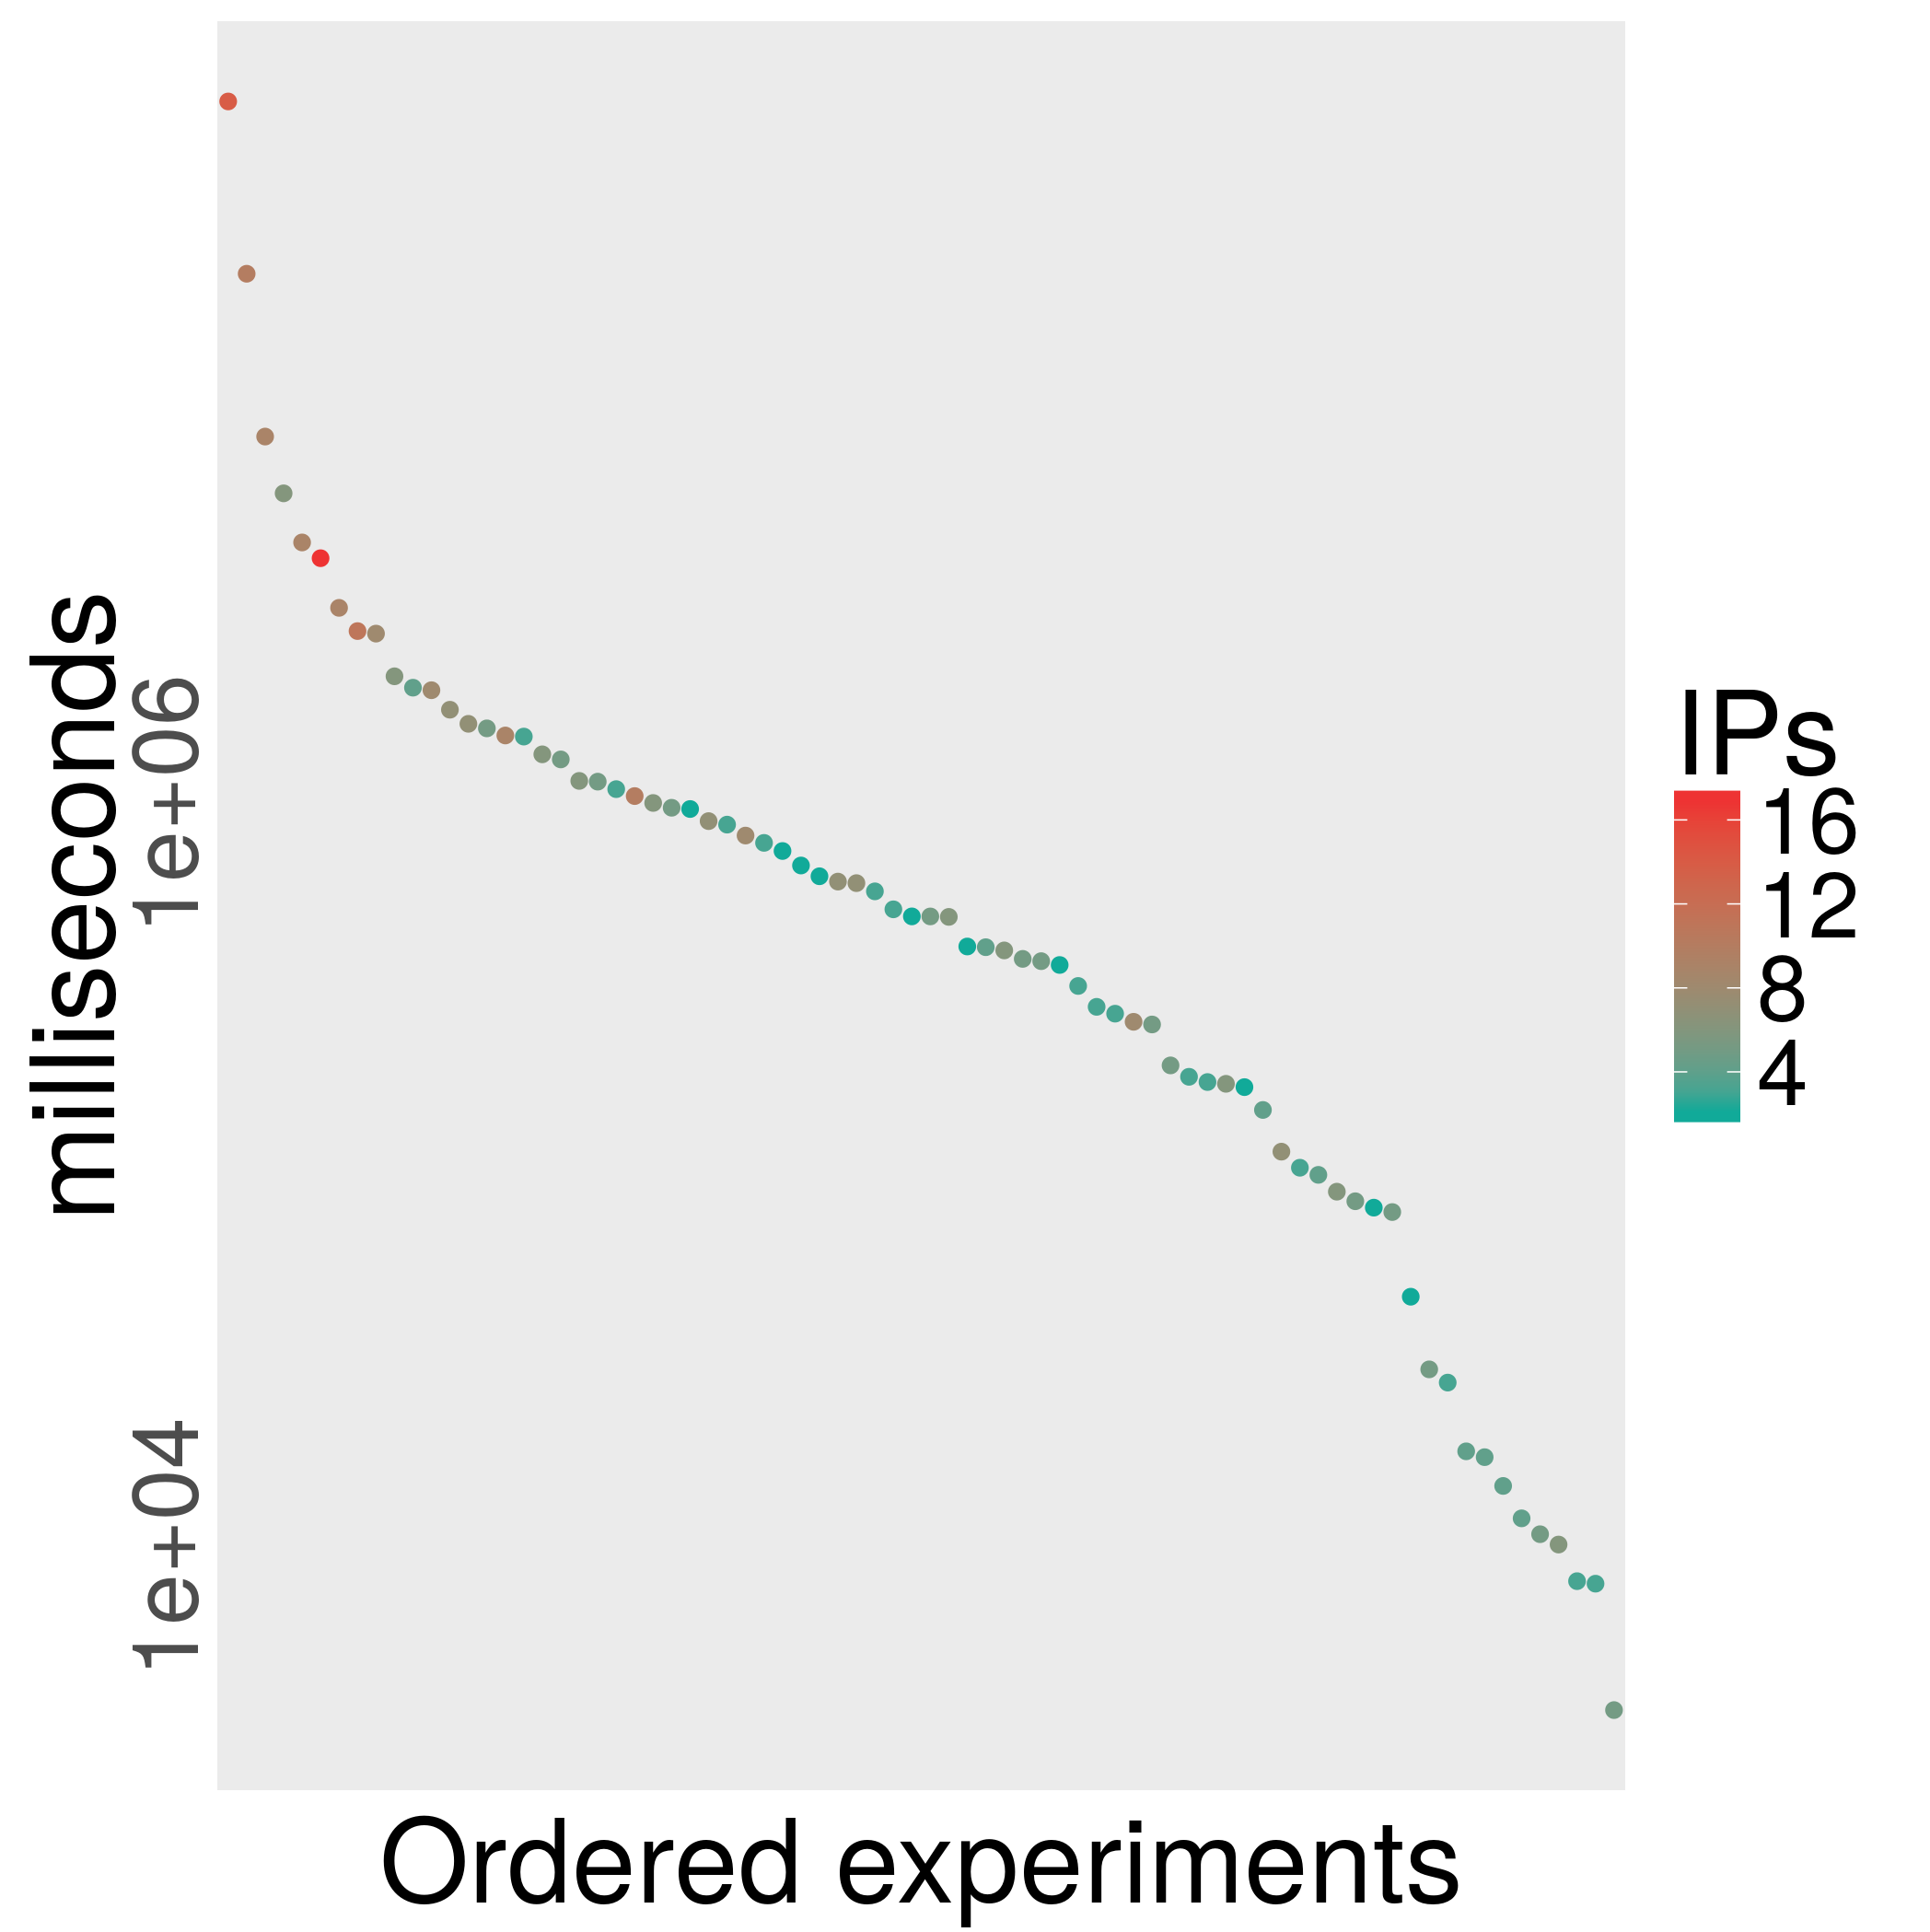
\includegraphics[width=0.32\linewidth]{time-vs-rank-alife-128.png}
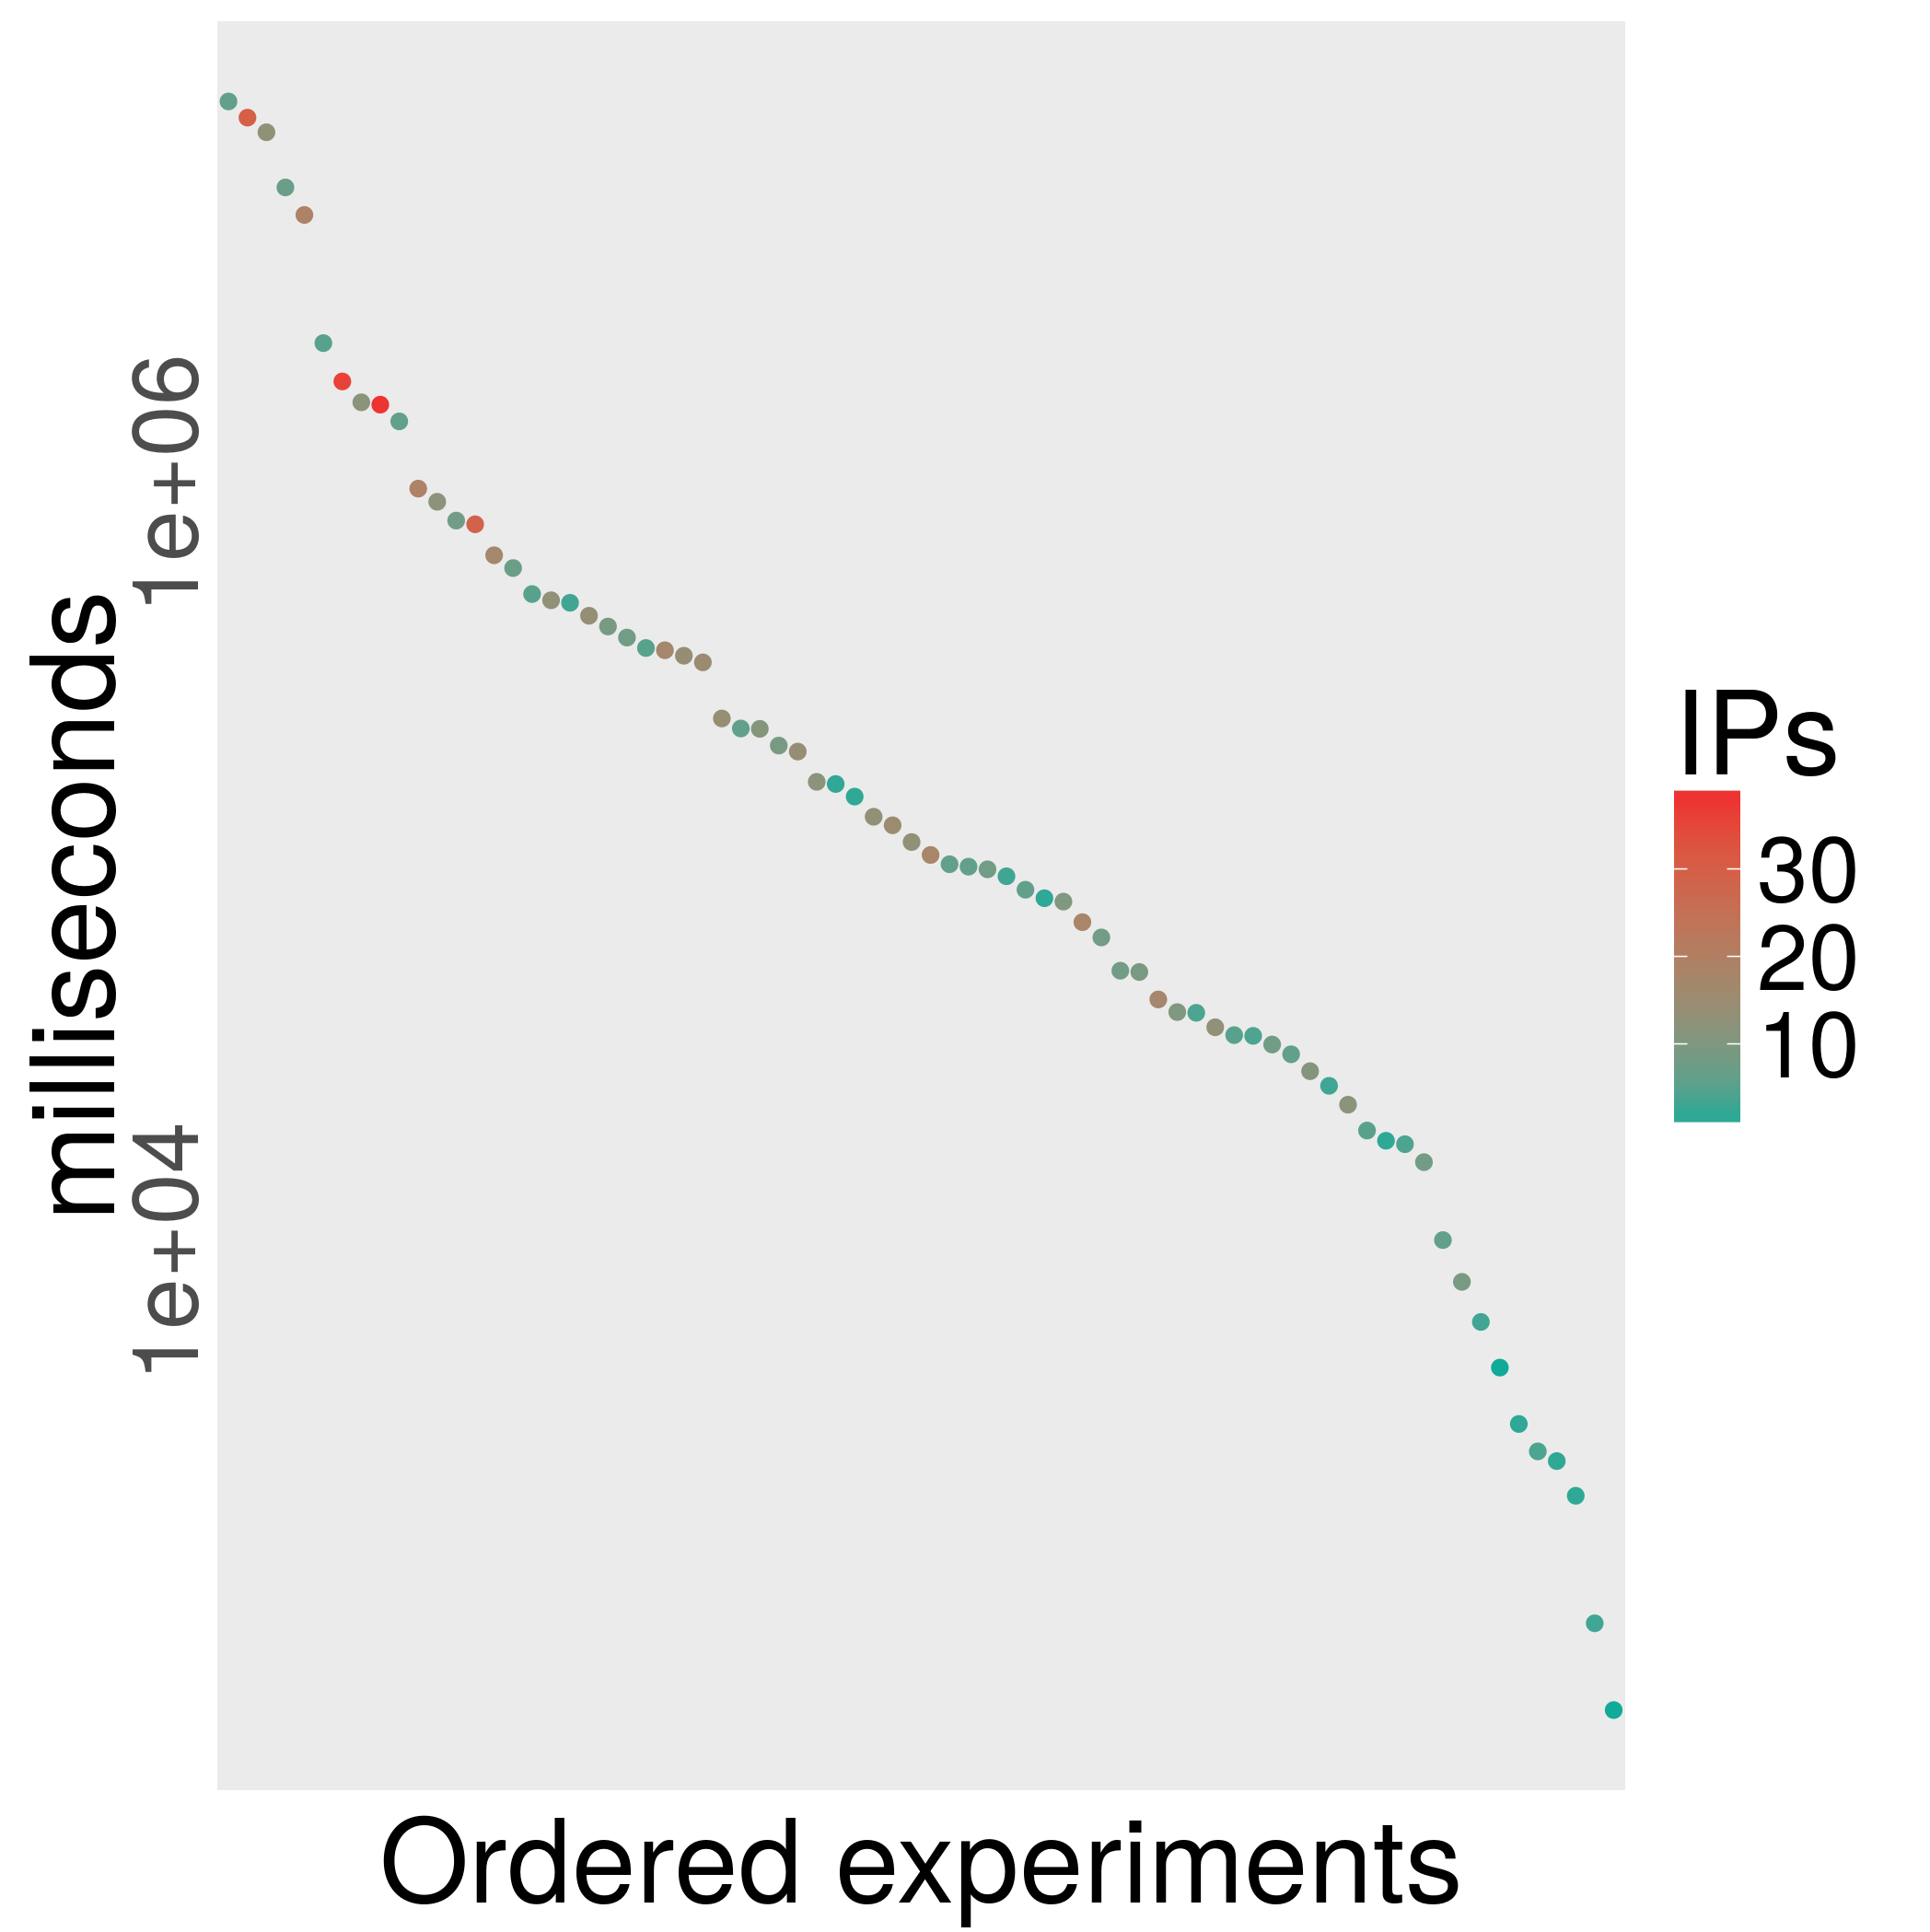
\includegraphics[width=0.32\linewidth]{time-vs-rank-alife-64.png}
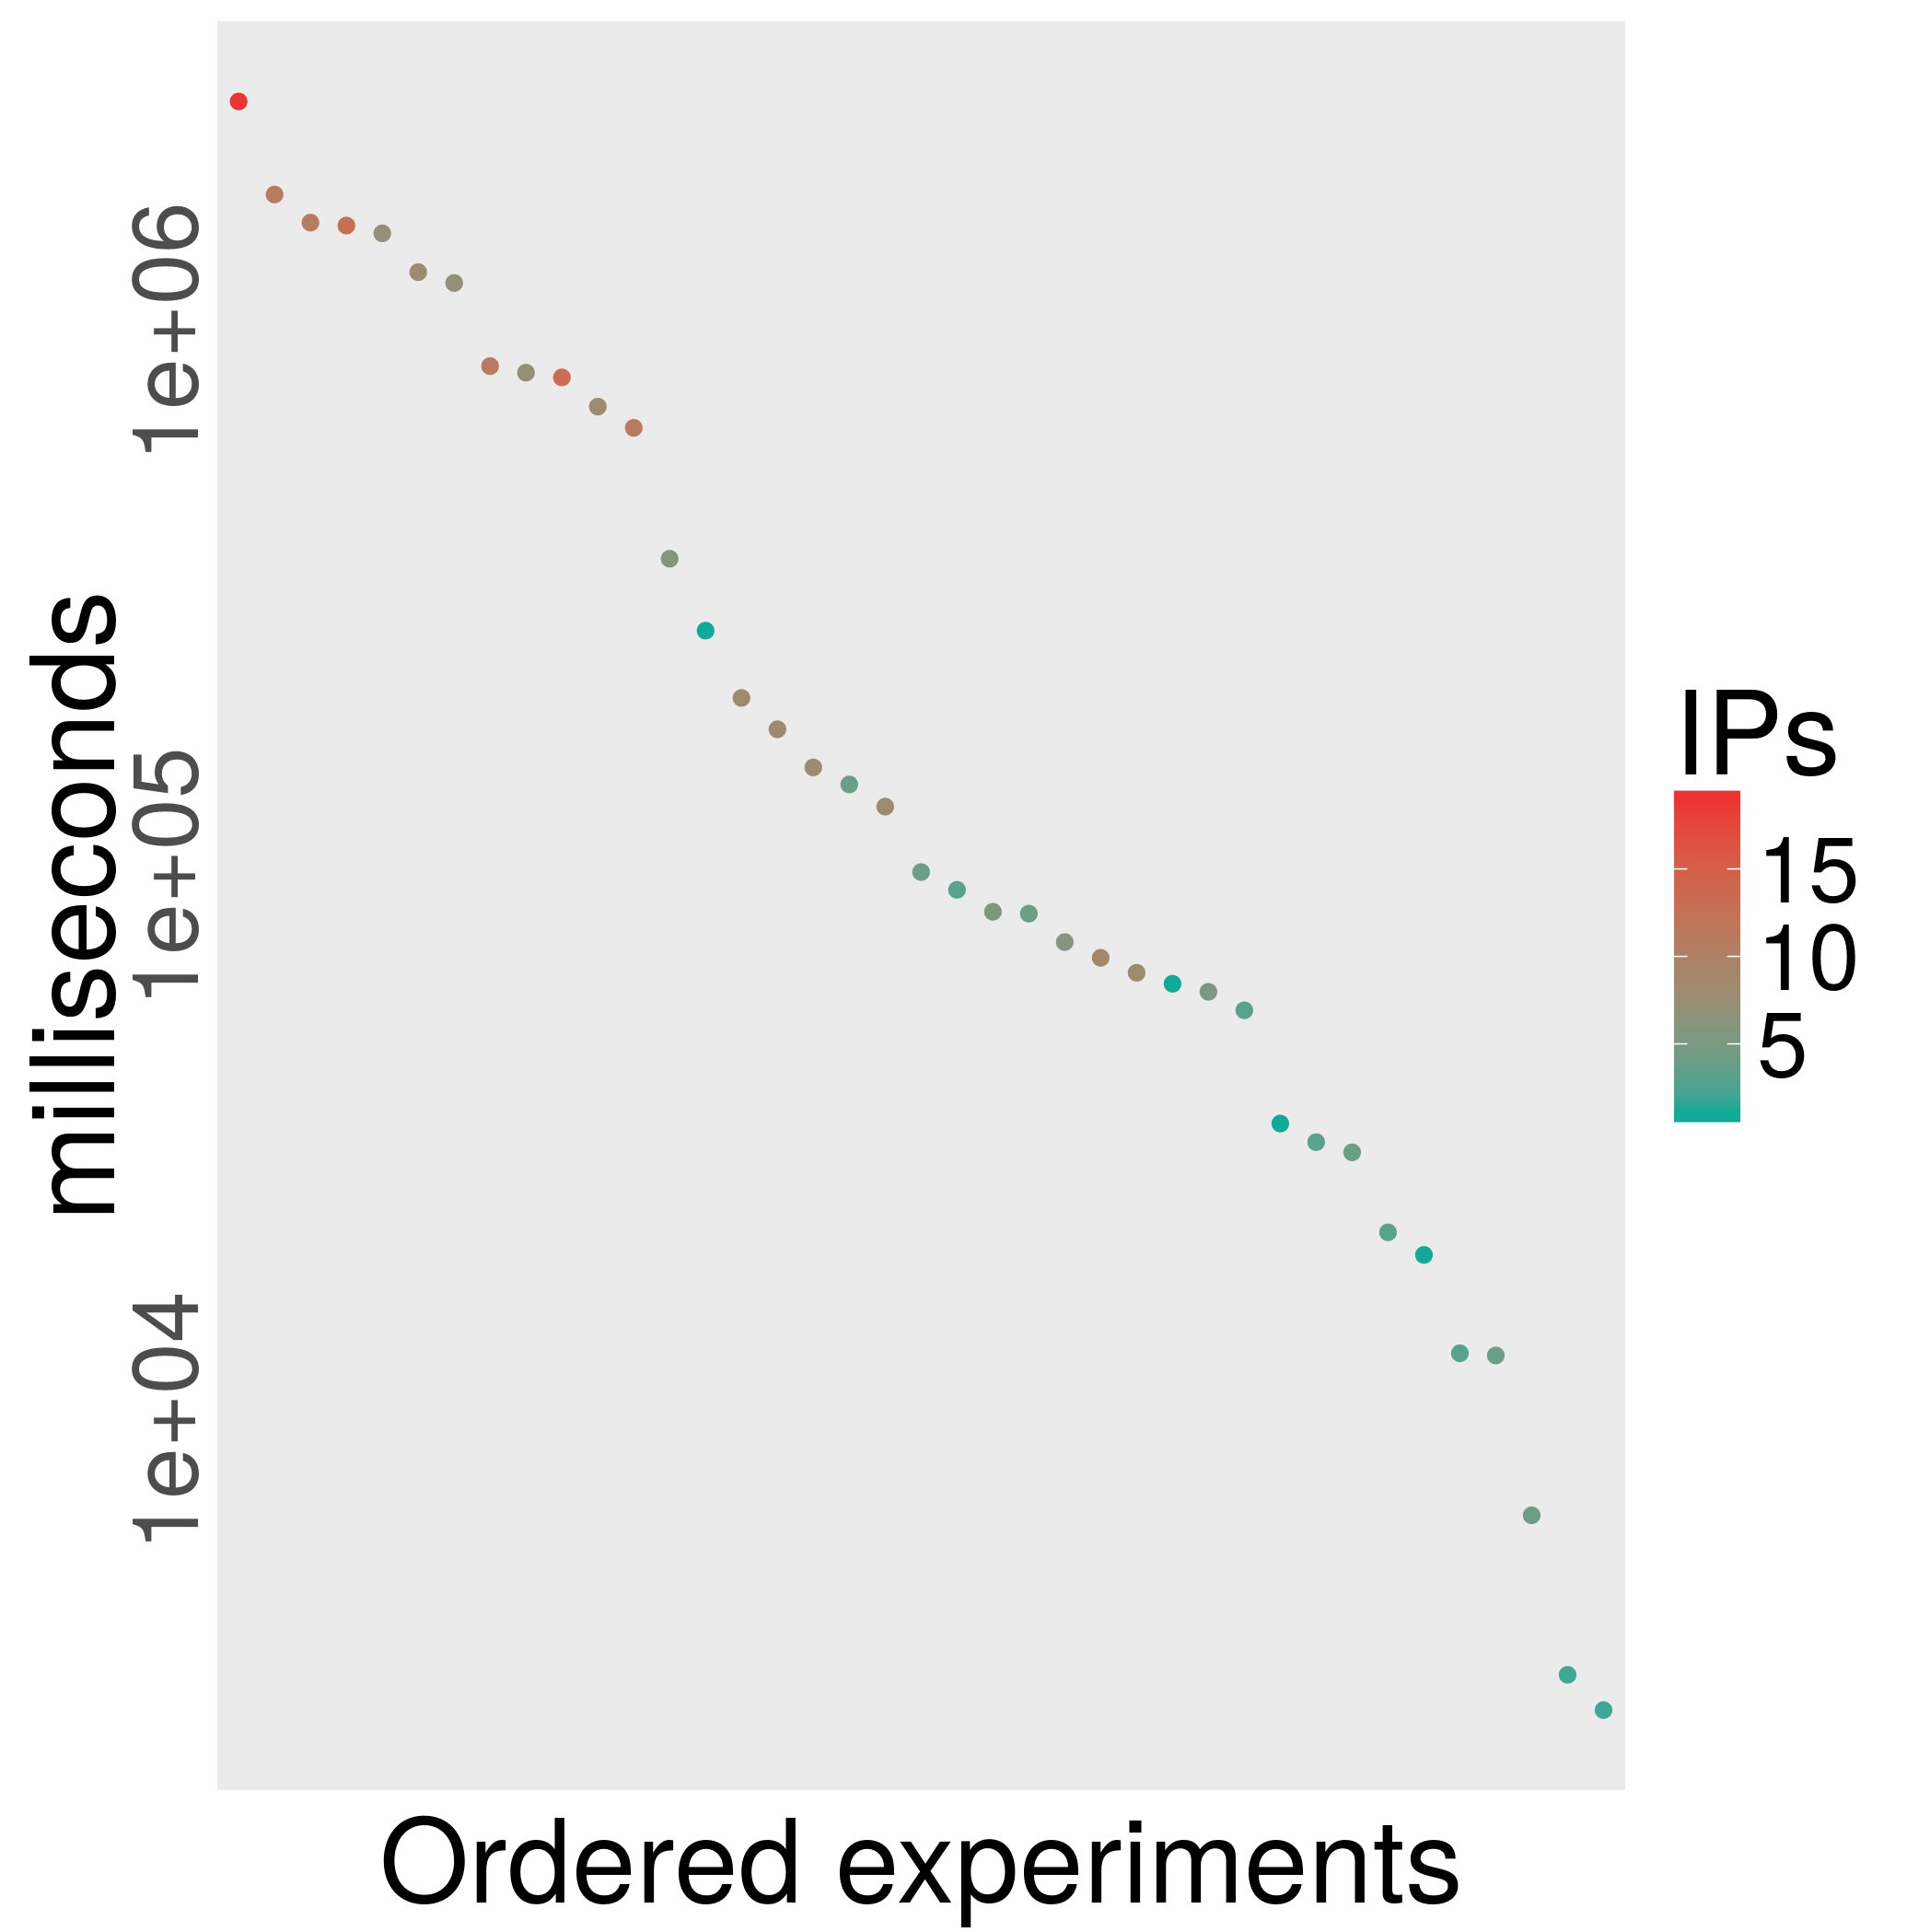
\includegraphics[width=0.32\linewidth]{time-vs-rank-alife-32.png}
\caption{Duration of experiments vs. rank, with $y$ axis in a
  logarithmic scale. Dot color is related to the number of IPs
  participating in the experiment. From left to right and top to bottom, experiments
  4/4, 4/24 and 7/31 and caches=128,64, 32} 
\label{fig:zipf:os}
% First ones made with time-vs-IPs-openshift.R:  
\end{figure}
%
It is also interesting to check the distribution of the experiment
duration, shown in Figure \ref{fig:zipf:os} and which roughly follows
a Zipf's law, with similar distribution along all three runs. The 4/24
run is the most complete and shows a S-shape, which implies an
accumulation of experiments taking similar time and around 100
seconds; this S-shape appears too in the experiments with cache=128
(bottom row, left). The most interesting part is the {\em tail}, which shows how
many experiments took a desirable amount of time, of the order of
10 seconds, and which appears in all three graphs. As it can be seen,
it sharply drops implying there are 
just a few of them, and with diminishing probability as time
decreases. However, since they have a greenish color, implying a low
number of IPs, they might be due to clients {\em carrying over} from
the previous one. This is a characteristic of this implementation
which will be examined later on, but at any rate if we discard those
experiments that take too much or too little, there is a decreasing
exponential distribution that corresponds to the Zipf's law.

\begin{figure}[!htb]
\centering
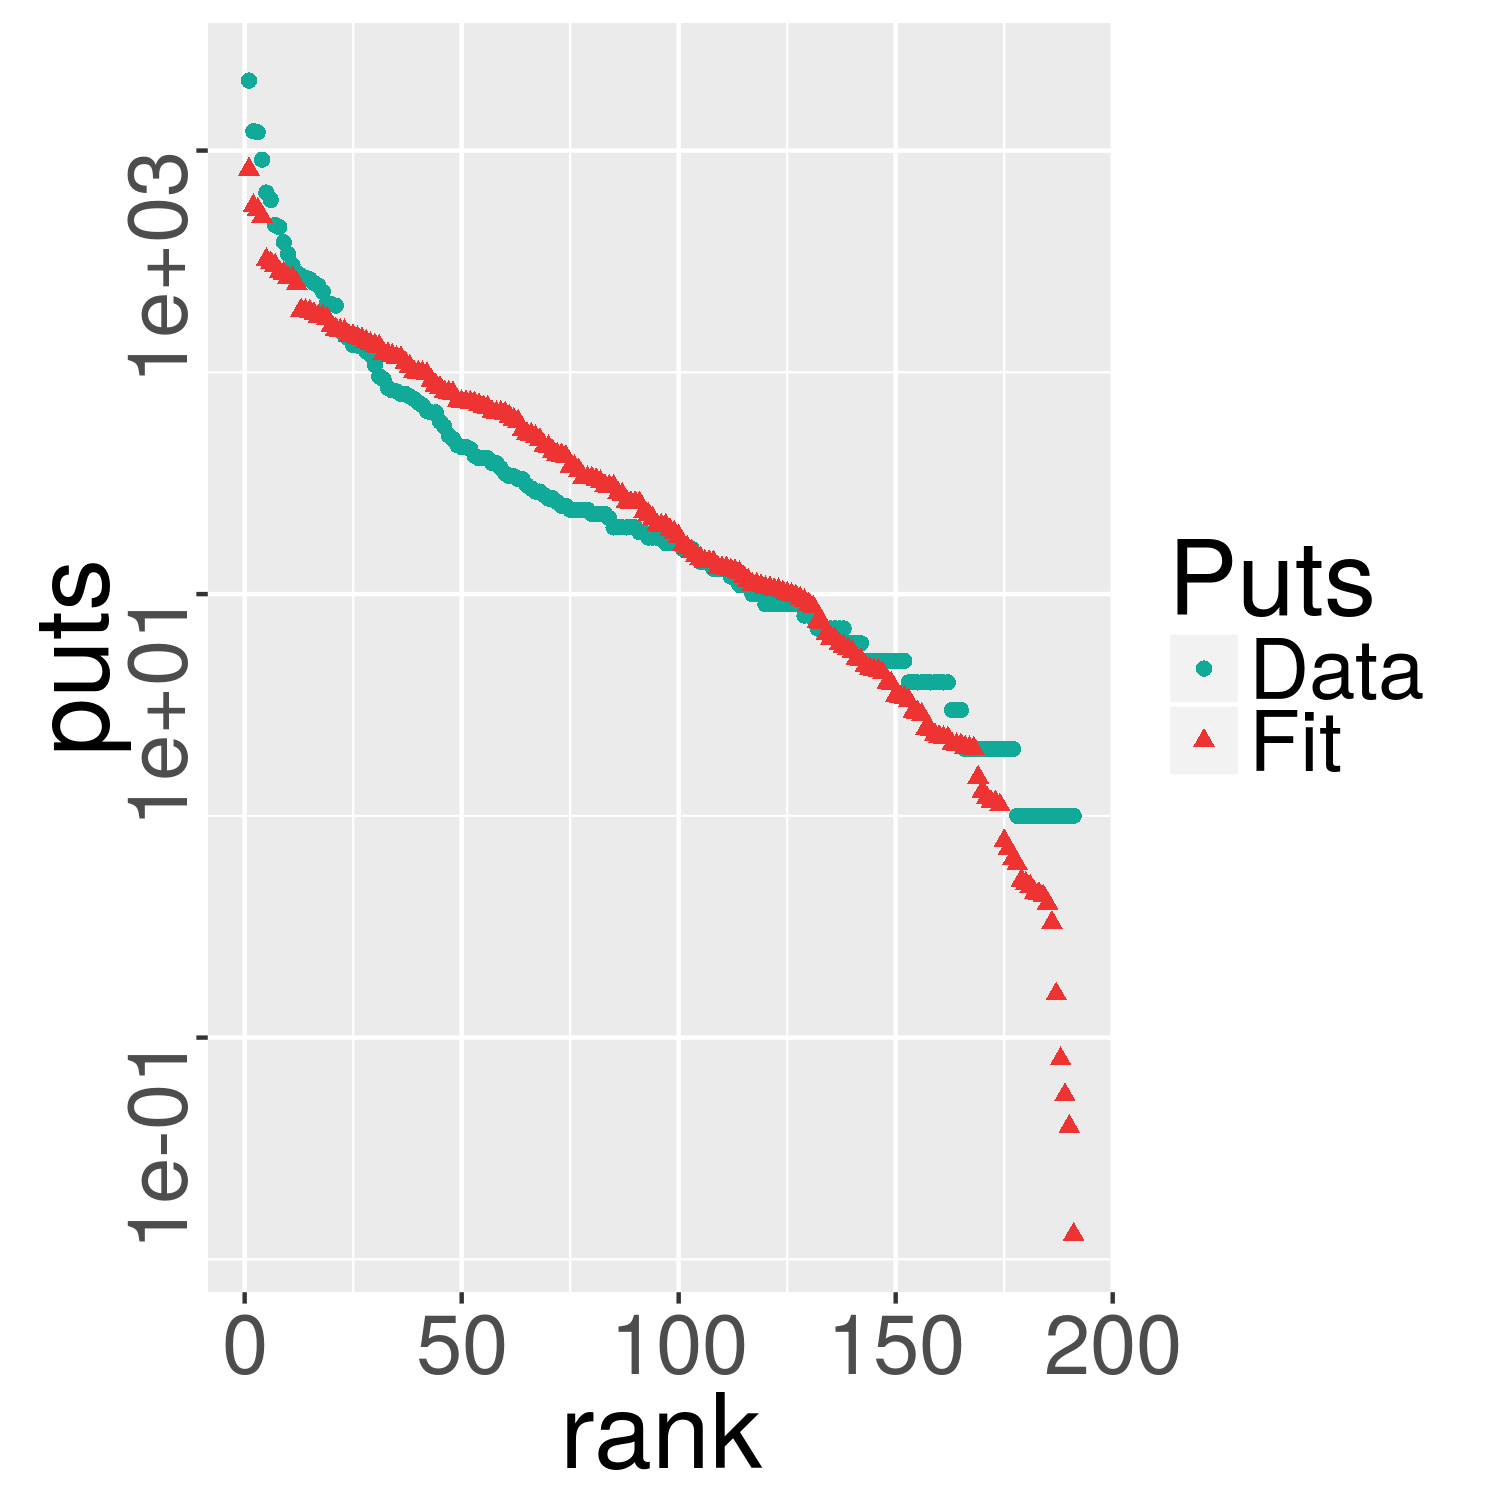
\includegraphics[width=0.32\linewidth]{weibull-puts-openshift-4-4.png}
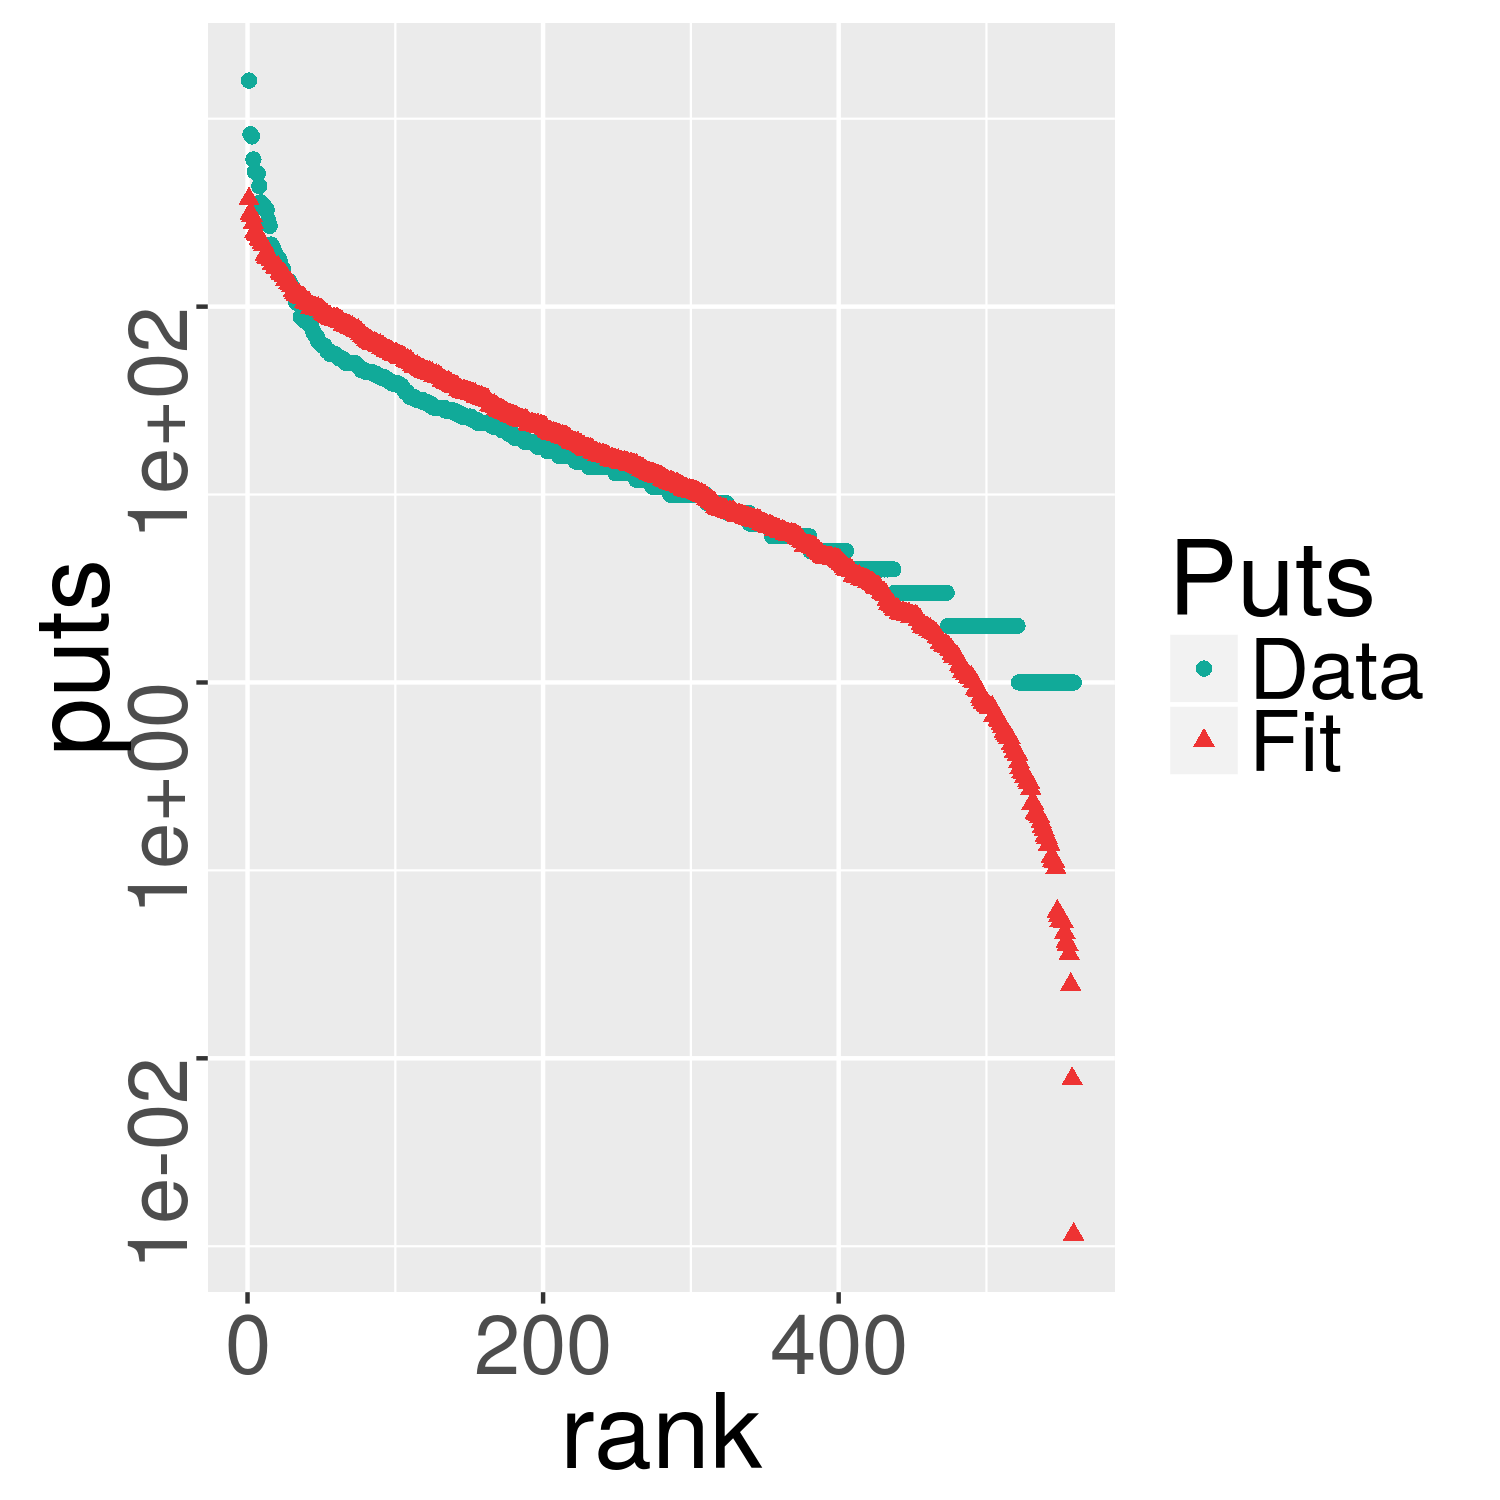
\includegraphics[width=0.32\linewidth]{weibull-puts-openshift-4-24.png}
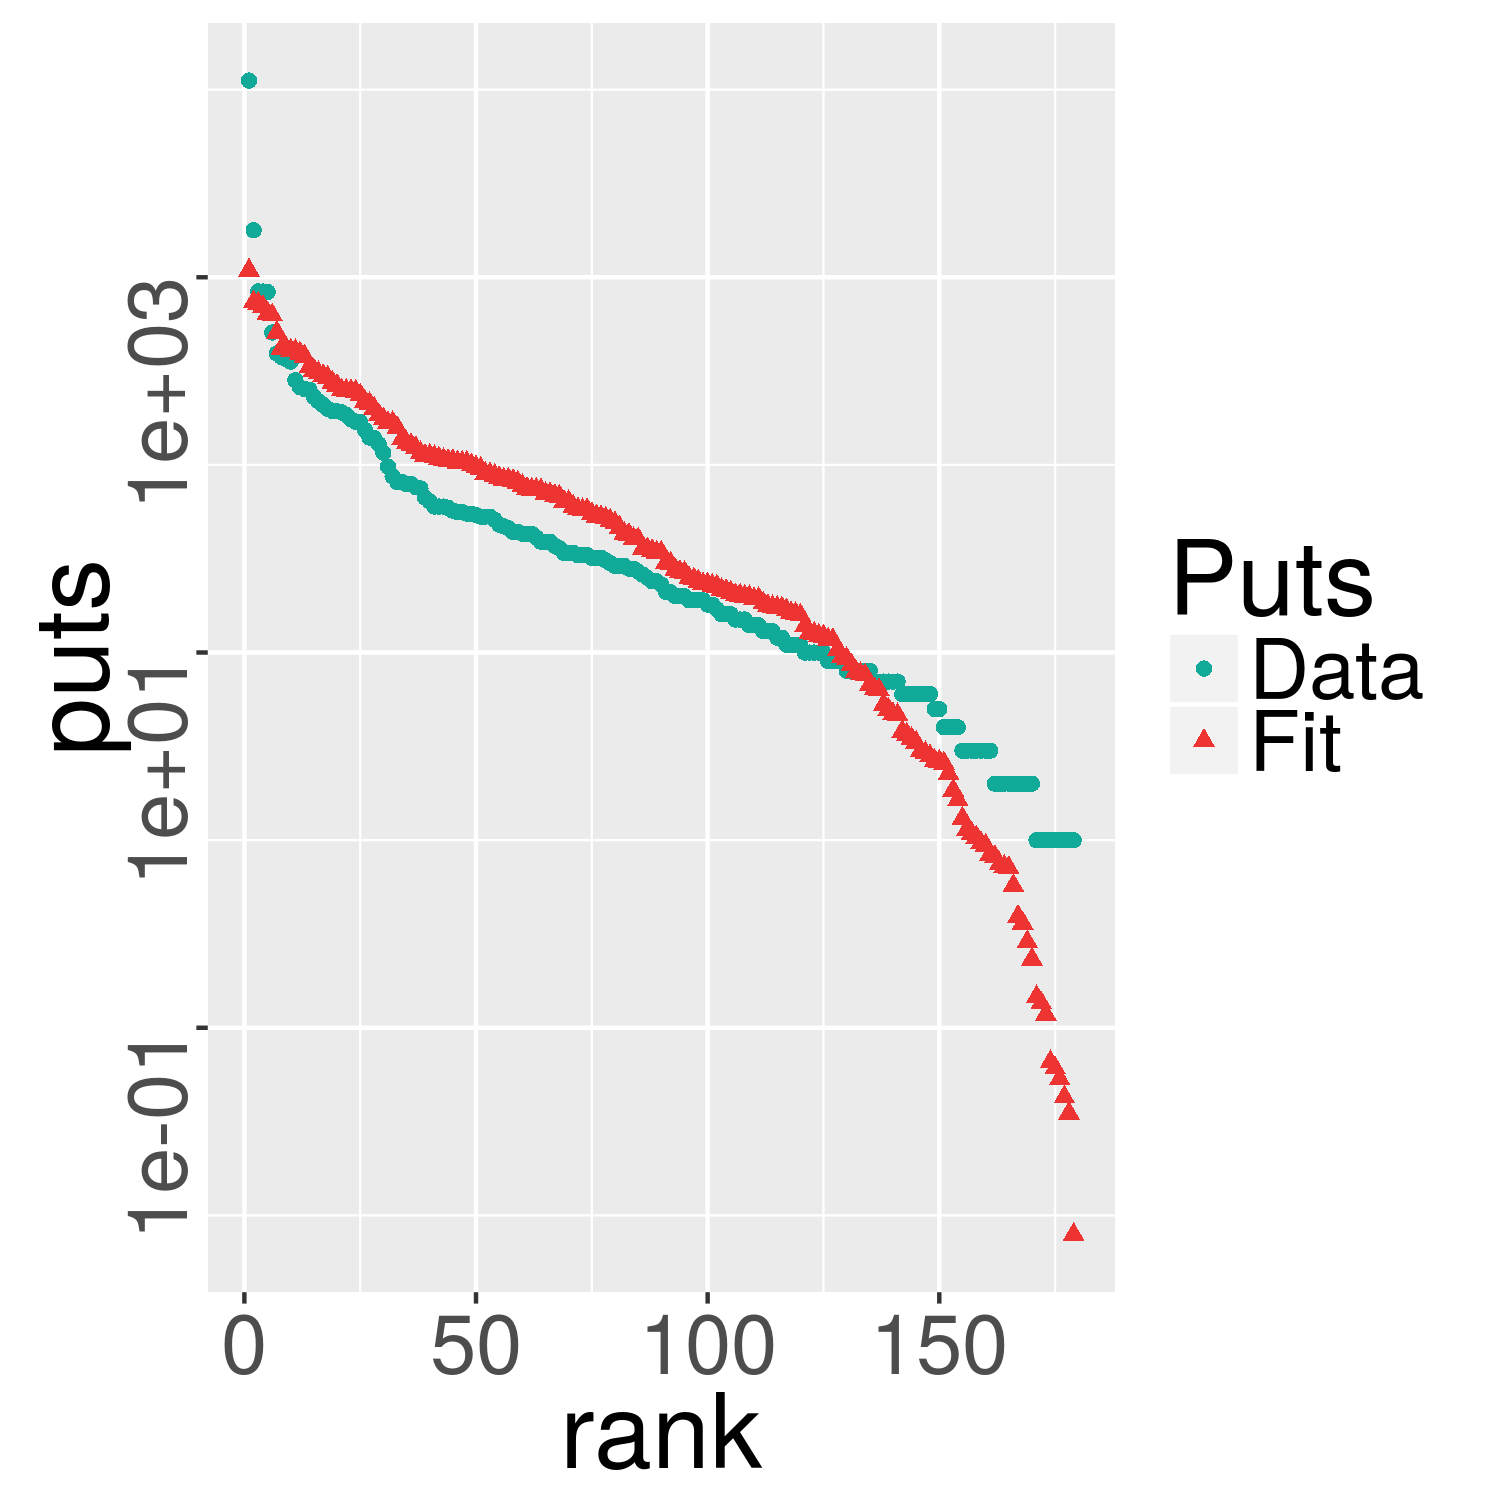
\includegraphics[width=0.32\linewidth]{weibull-puts-openshift-7-31.png}
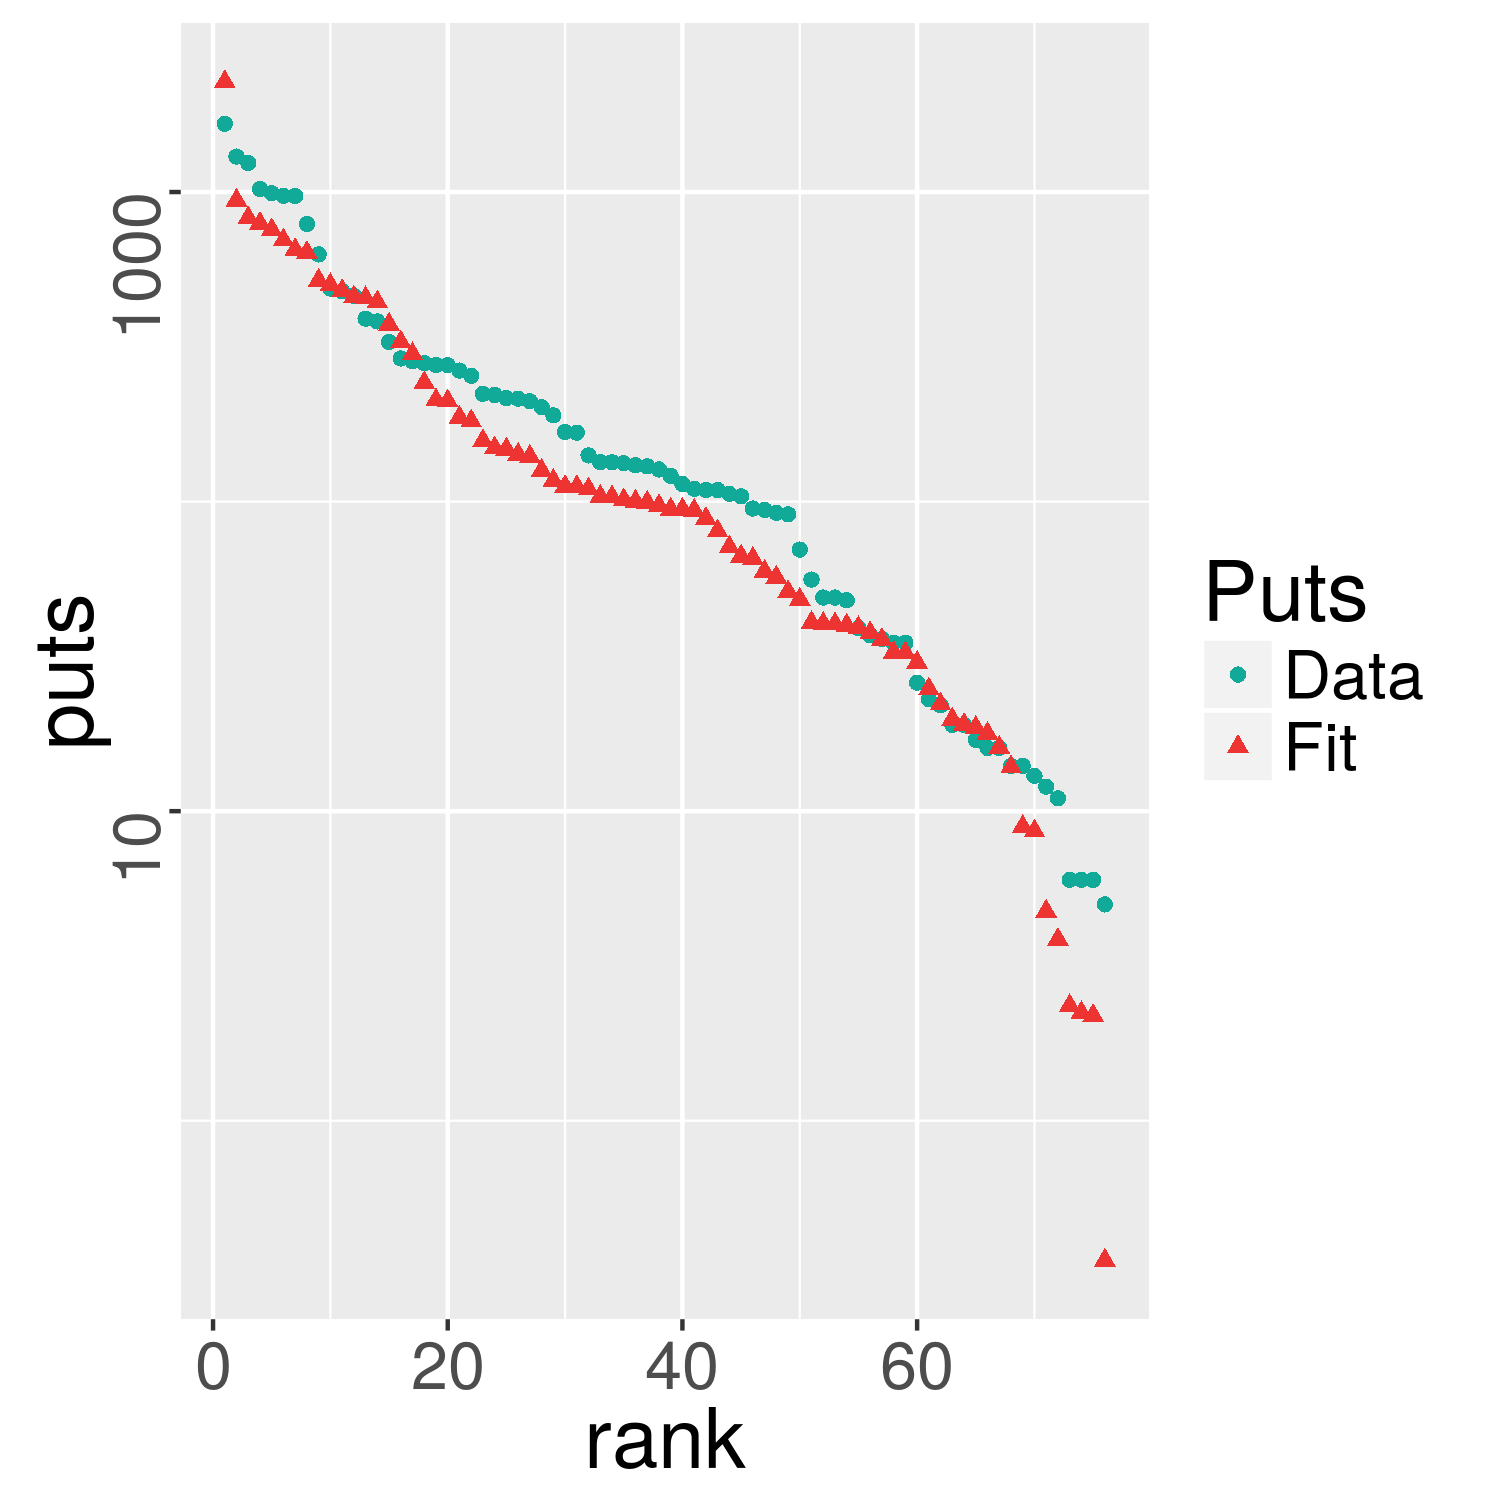
\includegraphics[width=0.32\linewidth]{weibull-fit-cache=128.png}
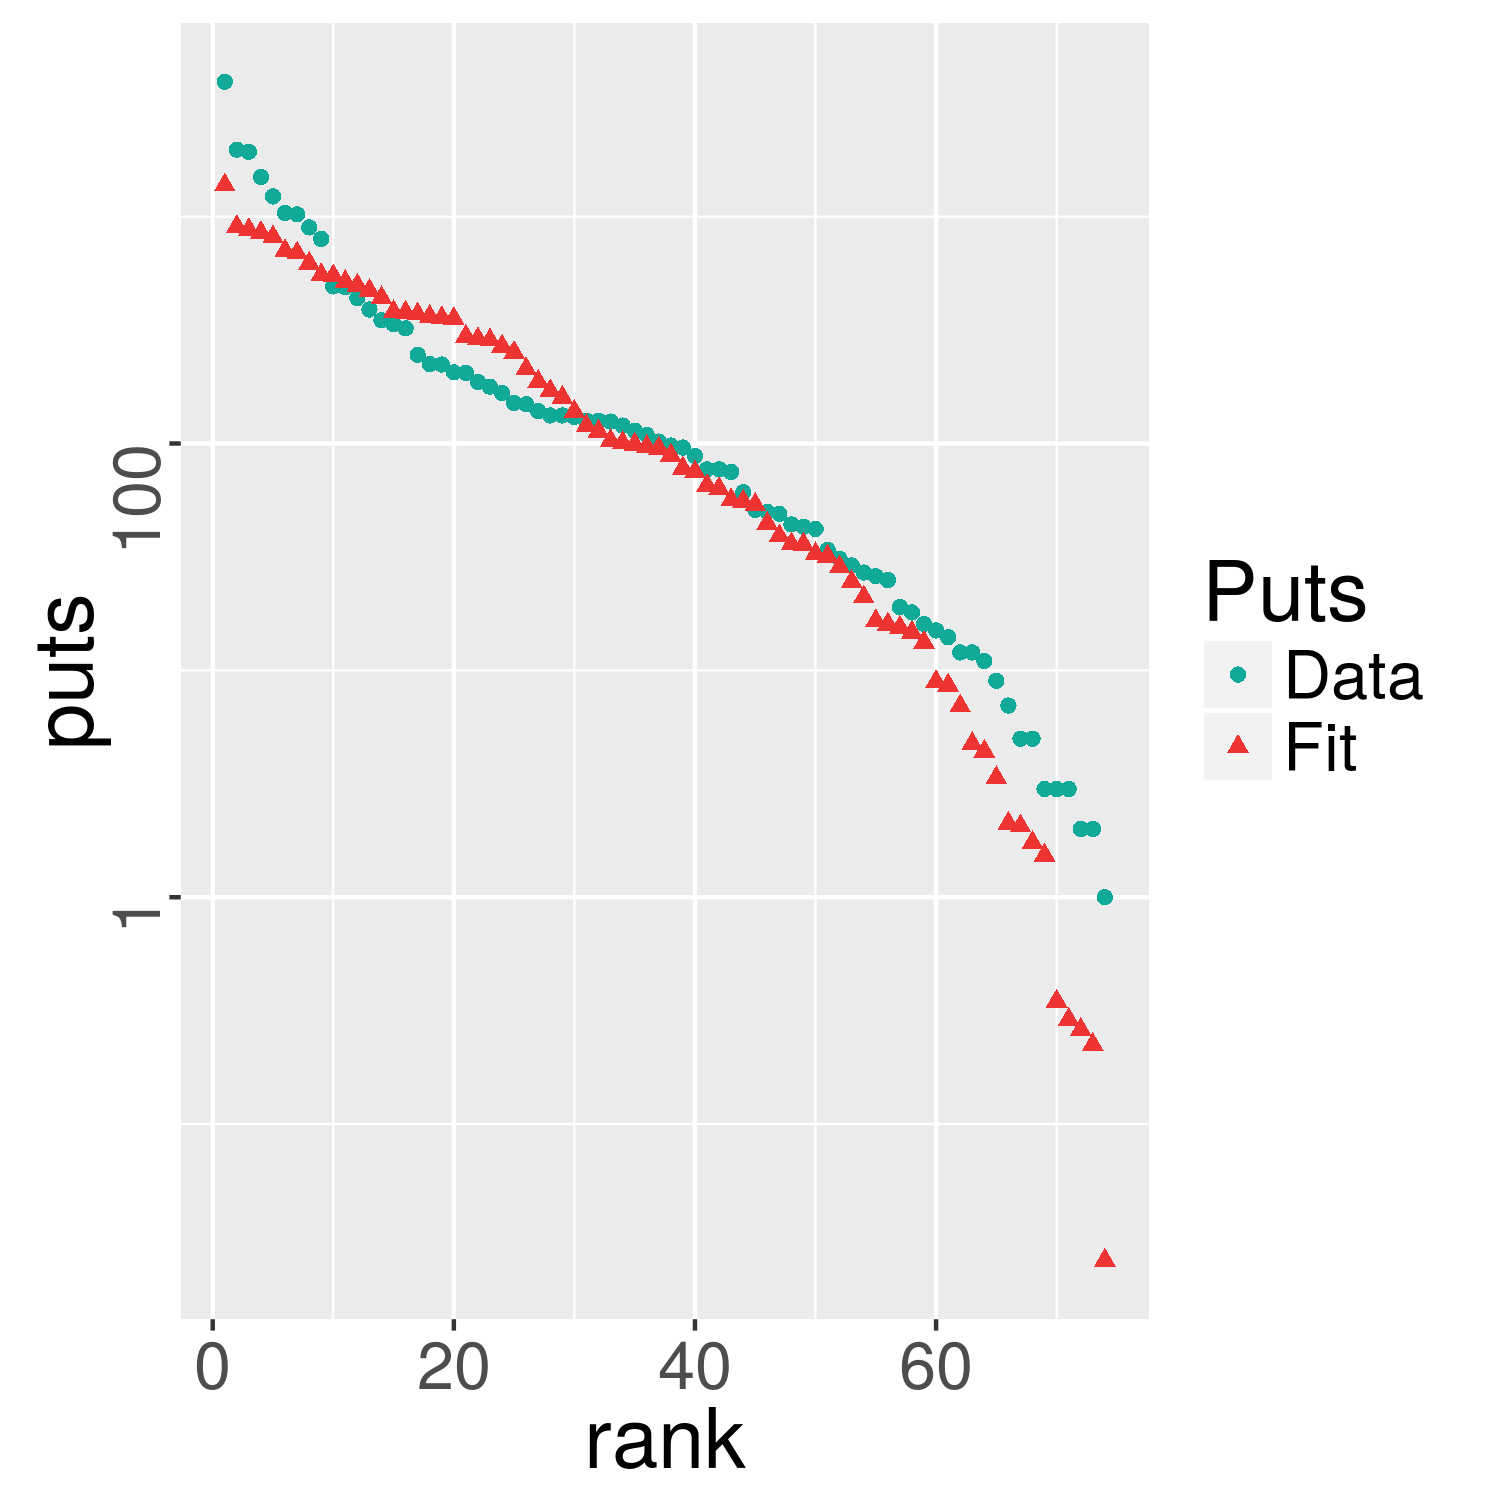
\includegraphics[width=0.32\linewidth]{weibull-fit-cache=64.png}
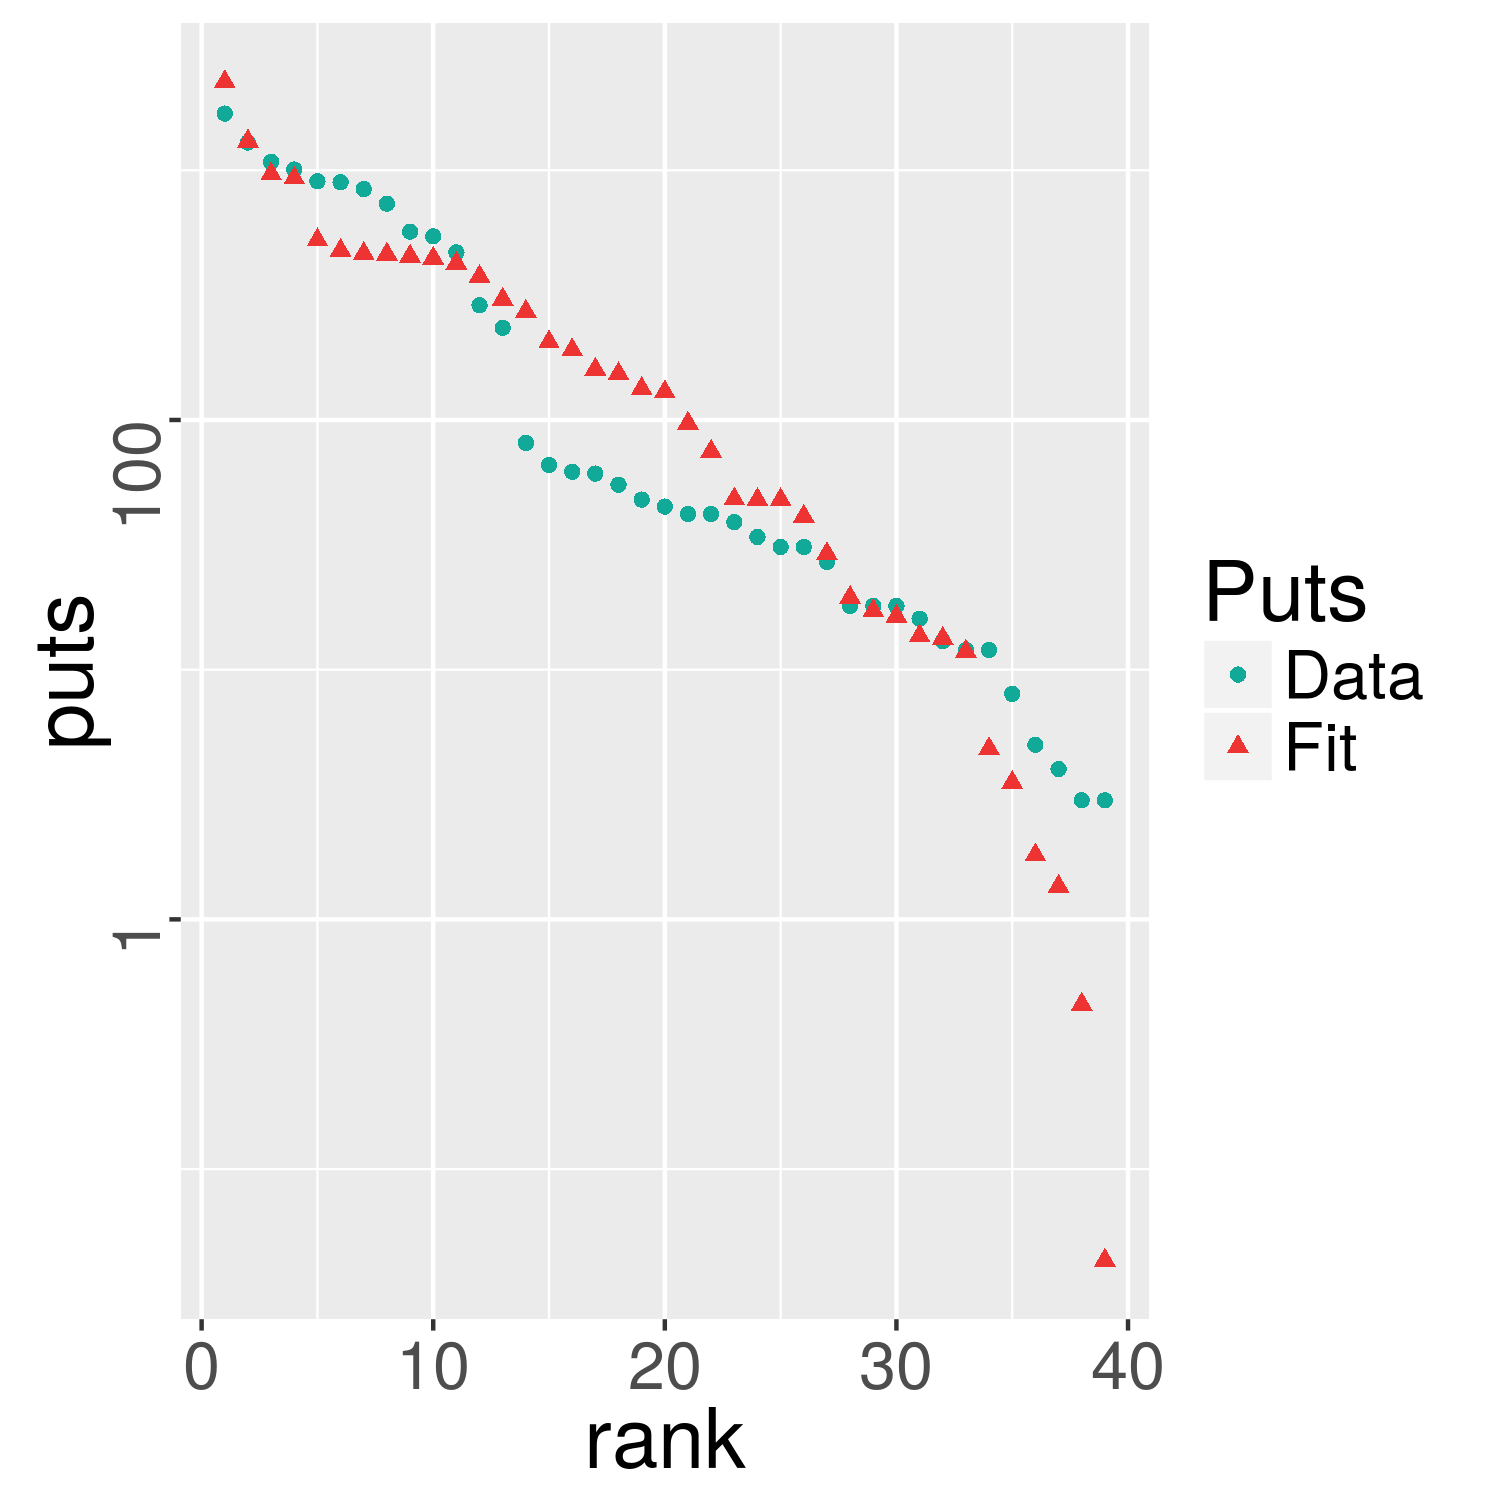
\includegraphics[width=0.32\linewidth]{weibull-fit-cache=32.png}
\caption{Number of {\tt PUT}s per unique IP and fit to a Weibull
  distribution (in red). From left to right and top to bottom, experiments
  4/4, 4/24 and 7/31 and new experiments with cache=128, 64, 32.} 
% Plotted with ../data/plot-zipf-openshift.R
\label{fig:puts:os}
\end{figure}
%
A similar exponential distribution also appears if we rank HTTP {\tt
  PUT}s, equivalents to the number of 
generations divided by 100, or to evaluations divided by 12800,
contributed by every user, which is shown 
in Figure \ref{fig:puts:os}. These results show a Zipf-like behavior,
that is, a power law with a small {\em bump} in the lowest
values. After testing the Generalized Extreme Value distribution and
failing for the new batch of experiments, we have fitted it to a
Weibull distribution \cite{thoman1969inferences} with the resulting
parameters shown in Table \ref{tab:puts:os}. 
%
\begin{table}
\caption{Weibull distribution  parameters of the fit of
  the number of {\tt PUT}s per unique IP. \label{tab:puts:os}}
\begin{center}
\begin{tabular}{l|cc}
\hline
Experiment  &  Scale $\sigma$ & Shape $\xi$ \\
\hline
4/4 &  43.07 $\pm$ 5.80 &  0.57 $\pm$ 0.03 \\
4/24 & 22.97 $\pm$ 1.57 & 0.66 $\pm$  0.02  \\
7/31 &  53.18 $\pm$ 7.77 &  0.54 $\pm$ 0.03   \\
\hline
Cache 128 & 205.28 $\pm$ 32.10 & 0.77 $\pm$ 0.07 \\ 
Cache 64 & 178.99 $\pm$ 36.44 & 0.60 $\pm$ 0.05 \\ 
Cache 32 & 168.15 $\pm$ 49.28 & 0.57 $\pm$ 0.07 \\
\hline
% from plot-zipf-openshift.R and ips-puts-alife.R
\end{tabular}
\end{center}
\end{table}
%
The inverse
Weibull distribution is a special case of the GEV distribution we have
used in those papers, and appears usually in natural sciences and
artificial life, usually related to decay. I has been frequently
fitted to volunteer computing frameworks such as SETI@home
\citep{javadi2009mining}. The model that user behavior follows can be
explained straighforwardly: when users visit the page, it draws their
attention for a limited amount of time. They give it a chance for a
few seconds. If something there amuses them or they can engage in a
conversation about it, they stay for a while longer, otherwise, they
leave. The {\em scale} parameter, which is around 20-40 in the first
batch for the 40 Trap problem and betwen 160 and 200 in the 60 traps
problem, depends mainly on the maximum number of generations people
leave it running. Since it finishes or stalls after a number of
generations shown in Figure \cite{tab:summary:os}, volunteer just
leave after that. Curiously enough, the scale parameter is roughly
twice the median number of {\tt PUT}s per experiment, showing that, on
average, the most loyal users reload the page twice after finishing or
after seeing the evolution does not progress. This rule of thumb
breaks down with the last experiment, however, which is interesting by
itself, too. 

The slope or shape parameter, on the other hand, indicates the overall
shape of the curve. A value less than 1 indicates a concave (in an
non-algorithmic scale) curve,
with figures closer to one indicating a smaller slope. In all cases
values are between 0.54 and 0.77, independently of the experiment. It
might be the case that this number depends more on the total number of
experiments carried out, with sets with more experiments, both in the
middle, having values between 0.60 and 0.70. The distribution is
remarkably similar which gives us a model of user behavior that is, to
a certain extent, independent of the experiment.  

These experiments show that, as it was proved for other volunteer
computer frameworks and also in the case of games, user engagement
follows a Weibull distribution. This makes engagement the key for
leveraging the performance of the sociotechnical metacomputer and a
way to improve results in the future. 

%---------------------------------------------------------------
\section{Conclusion}
\label{sec:conclusion}

In this paper two versions of a client-server architecture for volunteer and distributed
evolutionary algorithms that uses the browser and generated using {\sf
  NodIO}, based on the {\sf NodEO} evolutionary algorithm library have been
evaluated. Volunteers are {\em in the cloud}, as stated in the title,
since they are a {\em CPU as a service} for the persons running the
experiment. In fact, in this paper we have tried to put some figures
on the real size of that {\em cloud} and how it can be used standalone
if there is no alternative or in conjunction with other local or
cloud-based methods to add computing power in a seamless way through
the pool that NodIO creates. 

In order to establish a baseline performance, the evolutionary
algorithm was run in a desktop client-program written in JavaScript
using NodEO to solve the 40-trap function. The first experiments with
{\sf NodIO} proved that, although obtaining better performance than the
baseline was possible, it did not happen, mainly because of the
difficulty in carrying over volunteers to other experiments when the
one they were participating on was finished, shown in the low
correlation between the number of IPs in successive experiments. This
also resulted in a low number of generations allotted by users. 


The second objective of this paper was to model the user behavior in a
first attempt to try and predict performance. As should be expected,
the model depends on the implementation, with contributions following
a General Extreme Values distribution in the case of {\sf NodIO} and a
Weibull distribution for {\sf NodIO-W$^2$}. These distributions are
close enough to each other and, in the second case, reflect the fact
that all time spent in the page is actually devoted to computing,
which is why the time spent (represented by the number of
contributions to the pool) follows a model quite similar to that found
for games or other online activities. The reverse might be true: if we
want to have returning users for the experiments, it is probable that
we should {\em gamify} the experience so that once they've done it
once, they might do it more times. In the spirit of Open Science, this
gamification might involve computing in real time data such as the one
presented in this paper and showing it in the same page. 

In general, linking and finding correlations between user choices and
performance is an interesting avenue to explore in the future. Even if
the three previous experiments were published in a similar way, one
obtained up to 5 times more total cycles  than the one with the least
number of cycles. It is also essential to obtain volunteers as
simultaneously as possible, so it is possible that the features of the
social network in terms of real-time use will also play a big
role. Even as it is difficult to create controlled experiments in this
area, it is an interesting challenge to explore in the future.

Although we think that, in general, the results presented in this
paper are independent of the problem chosen, it is true that even if
it is a difficult problem for evolutionary algorithms, it takes a few
seconds with the right settings to solve. 
Besides, the two versions of the framework include as an
algorithmic variant using random population size. We do not think this
has had a big influence on the results and in fact this is not noticed
for F15, which is the second version tested but it would be interesting to
measure exactly what this influence has been. In general there are
many issues with the evolutionary algorithm implementation itself,
including using different, or adaptive, policies for inserting and
sending individuals to the pool,
using different policies for population initialization, and also the
incorporation of high-speed local resources to the pool to check what
would be the real influence of the volunteer pool to the final
performance. 

Another area is how to enhance the number and quality of
volunteers. For instance, adding a bit of more
control to the user might contribute also to gamification. Right now
the user has only two Web Workers. It is a matter of a single click to
open more tabs in the browser, giving more Web Workers, but it would be
interesting to put everything in a single page and under our control,
to check how often this happens and under which conditions. 

Finally, the implementation needs some refinement in terms of
programming and also ease of use. Tools such as Yeoman might be used % ¿añadir una cita o la URL http://yeoman.io/ a pie de página ?
to create a generator in which the user just has to create a fitness
function, with the rest of the framework wrapped around
automatically. All this, as the data used for this paper and the paper
itself, has been published with a free license in GitHub at
\url{https://github.com/JJ/modeling-volunteer-computing}.  

%---------------------------------------------------------------
\section*{Acknowledgments}

This work has been supported in part by TIN2014-56494-C4-3-P (Spanish Ministry of Economy and Competitivity),
PROY-PP2015-06 (Plan Propio 2015 UGR)  % please, remember to include all the current projects   ;)   Thanks!
. We would also like to thank the
anonymous reviewers of previous versions of this paper who have really
helped us to improve 
this paper (and our work) with their suggestions. We are also grateful
to Anna S\'aez de Tejada for her help with the data processing
scripts. We are also grateful to {\tt @otisdriftwood} for his help
gathering users for the new experiments. 


\bibliographystyle{apalike}
\bibliography{volunteer,GA-general,geneura,javascript,ror-js}

\end{document}

%%% Local Variables:
%%% ispell-local-dictionary: "english"
%%% End: